% Template:     Tesis LaTeX
% Documento:    Archivo principal
% Versión:      3.4.2 (07/02/2025)
% Codificación: UTF-8
%
% Autor: Pablo Pizarro R.
%        pablo@ppizarror.com
%
% Manual template: [https://latex.ppizarror.com/tesis]
% Licencia MIT:    [https://opensource.org/licenses/MIT]

% CREACIÓN DEL DOCUMENTO
\documentclass[
	spanish, % Idioma: spanish, english, etc.	
	letterpaper, oneside
]{book}

% INFORMACIÓN DEL DOCUMENTO
\def\documenttitle {Compresión de Atributos en Nubes de Puntos mediante Codificación Adaptativa Basada en Transformadas Dinámicas Dependientes de la Señal}
\def\documentsubtitle {}
\def\degreetitle {
	Tesis para optar al grado de magíster en ciencias de la ingeniería, mención eléctrica
	\bigbreak\vspace{0.3cm}
	
}

\def\universityname {Universidad de Chile}
\def\universityfaculty {Facultad de Ciencias Físicas y Matemáticas}
\def\universitydepartment {Departamento de la Universidad}
\def\universitydepartmentimage {departamentos/uchile2}
\def\universitydepartmentimagecfg {height=3cm}
\def\universitylocation {Santiago de Chile}

% INTEGRANTES, PROFESORES Y FECHAS
\def\documentauthor {Simón Yáñez Cárcamo}
\def\documentdate {\the\year}

\def\portrait {
	\begin{center}
	\vspace{1.5cm} ~ \\
	\MakeUppercase{\textbf{\documenttitle}} ~ \\
	\vspace{1.5cm}
	\MakeUppercase{\degreetitle} ~ \\
	\vfill
	\begin{tabular}{c}
		\MakeUppercase{\textbf{\documentauthor}} \\ \\
		\vspace{1.0cm} \\
		PROFESOR GUÍA: \\
		JORGE SILVA SÁNCHEZ\\
		\vspace{0.5cm} \\
		MIEMBROS DE LA COMISIÓN: \\
		EDUARDO PAVEZ CARVELLI \\
		PROFESOR 3 \\
		\vspace{0.5cm} \\
		Este trabajo ha sido parcialmente financiado por: \\
		AC3E \\
		\vspace{0.5cm} \\
		\MakeUppercase{\universitylocation} \\
		\MakeUppercase{\documentdate}
	\end{tabular}
	\end{center}
}
\def\abstracttable {
	\begin{tabular}{l}
		RESUMEN DE LA MEMORIA PARA OPTAR \\
		AL TÍTULO DE MAGÍSTER EN CIENCIAS \\
		DE LA INGENIERÍA \\
		POR: \MakeUppercase{\documentauthor} \\
		FECHA: \MakeUppercase{\documentdate} \\
		PROF. GUÍA: JORGE SILVA
	\end{tabular}
}

% IMPORTACIÓN DEL TEMPLATE
\input{template}

% INICIO DE LAS PÁGINAS
\begin{document}

% PORTADA
\templatePortrait

% CONFIGURACIÓN DE PÁGINA Y ENCABEZADOS
\templatePagecfg

% RESUMEN O ABSTRACT
\begin{abstractd}
Las nubes de puntos 3D son una herramienta fundamental para la representación de entornos complejos en aplicaciones como la realidad aumentada, la telepresencia y la navegación autónoma. Debido al crecimiento exponencial en la adquisición de datos 3D, se ha vuelto crítico desarrollar algoritmos de compresión eficientes, especialmente para los atributos como el color. Si bien el procesamiento de señales sobre grafos (GSP) ha permitido avances en la compresión de estos datos, las transformadas utilizadas suelen depender exclusivamente de la estructura geométrica, sin considerar la información contenida en la propia señal.

Este trabajo propone un enfoque novedoso basado en la construcción de transformadas gráficas adaptativas guiadas por la señal de color, lo cual permite representar de manera más compacta y eficiente la información contenida en bloques locales de la nube. A través de la introducción controlada de self-loops y la selección estratégica de bases, se busca optimizar la relación tasa-distorsión y minimizar el overhead asociado. Los resultados esperados incluyen mejoras cuantitativas y cualitativas frente al estado del arte, así como la implementación de un algoritmo completo y reproducible.
    
\end{abstractd}

% DEDICATORIA
\begin{dedicatory}
    Y es bueno vivir como se piensa, \\
    que de lo contrario pensarás como vives \\
	~ \\
	\textbf{Jose Pepe Mujica}
\end{dedicatory}

% AGRADECIMIENTOS
\begin{acknowledgments}
	PROXIMAMENTE
\end{acknowledgments}

% TABLA DE CONTENIDOS - ÍNDICE
\templateIndex

% CONFIGURACIONES FINALES
\templateFinalcfg

% ======================= INICIO DEL DOCUMENTO =======================

\chapter{Introducción}

Las \textit{nubes de puntos 3D} constituyen una representación eficiente y flexible para describir objetos, personas y entornos tanto interiores como exteriores. Estas representaciones tienen aplicaciones clave en campos como la realidad aumentada y virtual (AR/VR), la telepresencia y los vehículos autónomos. Una nube de puntos 3D está compuesta por una lista de coordenadas espaciales acompañadas de atributos asociados, siendo el color uno de los más comunes.

Gracias a los recientes avances tecnológicos, este tipo de datos puede capturarse en alta resolución, en tiempo real y a bajo costo, utilizando sensores \textit{LiDAR} integrados en dispositivos móviles o vehículos. Esta facilidad de adquisición ha llevado a una rápida proliferación de datos 3D, lo que ha motivado el desarrollo de técnicas de compresión eficientes, tanto para la geometría como para los atributos de color de las nubes de puntos~\scite{loop2016microsoft}.
\\

En imágenes y video tradicionales, la compresión con pérdida se realiza eficientemente mediante procesamiento por bloques y transformadas como la \textit{Discrete Cosine Transform} (DCT)~\scite{chen1975enhancement}, utilizada en estándares como \textit{JPEG}~\scite{jpeg1992}. Sin embargo, las nubes de puntos presentan una geometría irregular, desordenada y carente de estructura temporal coherente, lo que impide la aplicación directa de técnicas convencionales.
\\

Ante este desafío, el procesamiento de señales sobre grafos (\textit{Graph Signal Processing}, GSP) ha emergido como una herramienta poderosa para tratar datos no estructurados como las nubes de puntos. Mediante la construcción de grafos según reglas simples, es posible dotar de estructura a estos datos y procesarlos como señales definidas sobre vértices.
\\

Actualmente, esta perspectiva se ha aplicado en compresión mediante el uso de la transformada de Fourier sobre grafos (GFT), estableciendo un claro paralelismo con la DCT en el contexto de señales clásicas~\scite{ortega2022gsp}. A partir de esta base, se han propuesto múltiples variantes orientadas a minimizar la tasa de bits requerida y la distorsión introducida, priorizando la conservación de la información visualmente más relevante~\scite{pavez2020region}. Sin embargo, dichas técnicas suelen centrarse en reglas estructurales de la nube para comprimir el espacio de color, sin explorar en profundidad el uso de la señal misma para construir bases más compactas e informativas.
\\

En esta investigación se plantea la hipótesis de que, al analizar el comportamiento del espacio de color, es posible construir estructuras matemáticas adaptativas que permitan una compresión más eficiente. Se propone generar un conjunto de transformadas personalizadas, donde a nivel de bloques se puedan tomar decisiones óptimas~\scite{ortega1998rate} en función de la tasa, la distorsión y el \textit{overhead}. Como resultado, se desarrollará un algoritmo completo capaz de aprovechar la información contenida en el color para lograr una compresión de mayor calidad y menor tamaño.

\section{Justificación}

La creciente disponibilidad de sensores 3D de bajo costo ha permitido la adquisición masiva de nubes de puntos en diversas aplicaciones prácticas. Sin embargo, este avance también ha generado desafíos significativos en términos de almacenamiento, transmisión y procesamiento eficiente de grandes volúmenes de datos. La compresión efectiva de estos datos es, por tanto, una necesidad urgente para garantizar su escalabilidad en contextos como la realidad aumentada, la telepresencia o los sistemas de navegación autónoma.

A diferencia de las imágenes tradicionales, las nubes de puntos no cuentan con una estructura regular subyacente, lo que impide la aplicación directa de técnicas de compresión convencionales. Aunque las herramientas del procesamiento de señales sobre grafos han mostrado avances notables~\scite{ortega2022gsp}, la compresión de atributos como el color sigue siendo limitada por el uso de heurísticas estructurales generales, sin aprovechar completamente la información contenida en la señal misma.

Esta investigación busca abordar esa brecha mediante el diseño de transformadas informadas por el comportamiento de la señal de color, lo que no sólo puede mejorar la eficiencia de la compresión, sino también ofrecer una alternativa adaptable, interpretable y más alineada con la naturaleza del contenido visual.

\section{Objetivos}

\textbf{Objetivo general:}

\begin{itemize}
    \item \textit{Desarrollar un algoritmo de compresión para los atributos de nubes de puntos dependientes de la señal, adaptativo y superior al estado del arte de manera cuantitativa y cualitativa.}
\end{itemize}

\textbf{Objetivos específicos:}

\begin{itemize}
    \item \textit{Explorar y entender las técnicas de transform based coding aplicadas al contexto de Graph Signal Processing.}
    \item \textit{Estudiar y proponer herramientas matemáticas para la representación de la dinámica de los atributos de color.}
    \item \textit{Observar, analizar e implementar experimentos sobre el efecto de los self-loops en la construcción de bases.\scite{pavez2017separable}}
    \item \textit{Plantear y visualizar la ganancia en tasa-distorsión de la implementación estratégica de self-loops mediante estrategias de optimización por bloques.}
    \item \textit{Estudiar la distribución de las decisiones y el overhead de las instrucciones de las transformadas alcanzadas.}
    \item \textit{Plantear un algoritmo final de compresión cuya ganancia sea demostrable y competitiva frente al estado del arte.}
\end{itemize}

\section{Metodología general}

Para abordar este problema, se propone un enfoque basado en el diseño de transformadas adaptativas a nivel de bloques, cuya construcción se guía por la distribución del color en cada segmento. A partir de reglas heurísticas y métricas de tasa-distorsión, se evaluarán variantes estructurales que permitan identificar bases eficientes para la compresión. Los experimentos incluirán comparaciones con métodos gráficos tradicionales, utilizando métricas estándar de compresión y calidad visual. Se realizarán validaciones cuantitativas (PSNR, bitrate) y cualitativas (análisis perceptual) en conjuntos de datos sintéticos y reales.

\section{Contribuciones esperadas}

\begin{itemize}
    \item \textit{Propuesta de un esquema de compresión adaptativo que explota la dinámica local del espacio de color.}
    \item \textit{Desarrollo de nuevas variantes de transformadas gráficas construidas a partir de la señal, no sólo de la estructura.}
    \item \textit{Estudio sistemático del efecto de self-loops en la compacidad de la representación espectral.}
    \item \textit{Implementación de un algoritmo completo de compresión de atributos, con mejoras comprobables frente a métodos existentes.}
    \item \textit{Generación de código abierto con documentación técnica para su reproducción y uso en futuras investigaciones.}
\end{itemize}
 % Ejemplo, se puede borrar
\chapter{Marco Teórico}

En este capítulo se profundizarán los conceptos y conocimientos que sustentan el desarrollo de esta tesis. Fundamentalmente, se explorarán y analizarán los campos y elementos que han sido utilizados directa o indirectamente para el cumplimiento de los objetivos planteados.

Los conceptos presentados a continuación son esenciales para comprender los métodos de compresión y, por ende, para entender el método propuesto en esta investigación. En esta sección se detallarán nociones propias de la teoría de la información desde su paradigma clásico. Posteriormente, a partir de estos conceptos generales, se abordarán las adaptaciones y analogías correspondientes al paradigma de grafos. Estos conceptos son clave para entender la lógica y motivación del algoritmo propuesto, así como para fundamentar las métricas de desempeño que validan el cumplimiento de los objetivos de este trabajo.

\section{Fundamentos de Teoría de la Información}

Al abordar métodos de compresión, es imprescindible partir de ciertos fundamentos esenciales de la teoría de la información. Esta disciplina proporciona el marco matemático necesario para definir, medir y manipular la información contenida en una fuente, y toda técnica de compresión se construye sobre estos principios fundamentales \cite{mackay_nodate, sayood2006introduction}.

El primer concepto clave es el de \textit{auto-información}, que representa la cantidad de información que aporta un evento al ocurrir. Matemáticamente, se define como:

\begin{equation}
i(A) = \log_b \frac{1}{P(A)} = -\log_b P(A)
\end{equation}

Esta expresión refleja la intuición de que un evento raro contiene más información que uno común. El logaritmo actúa de manera inversa a la probabilidad, de modo que cuanto menos probable es un suceso, mayor es su auto-información. En términos intuitivos, se puede pensar que una lluvia en el desierto informa más que una lluvia en una ciudad lluviosa: lo inesperado comunica más \cite{mackay_nodate}.

Cuando la fuente está compuesta por varios eventos posibles $A_i$, cada uno con probabilidad $P(A_i)$, la información promedio que entrega dicha fuente se calcula como una suma ponderada de auto-informaciones, a la que se denomina \textit{entropía}:

\begin{equation}
H = -\sum_i P(A_i) \log_b P(A_i)
\end{equation}

La entropía mide la incertidumbre promedio de la fuente. Shannon demostró que esta cantidad representa el límite inferior teórico del número de bits necesarios para codificar la salida de una fuente sin pérdida \cite{sayood2006introduction, mackay_nodate}. Esto implica que ningún esquema de codificación sin pérdida puede, en promedio, superar la compresión indicada por $H$.

Si se dispone de información adicional sobre el contexto de la fuente, es posible reducir aún más esta incertidumbre. Esta idea se formaliza mediante la \textit{entropía condicional}, que mide la incertidumbre de una variable $X$ dado que se conoce otra variable $Y$ relacionada:

\begin{equation}
H(X|Y) = -\sum_{x,y} P(x, y) \log_b P(x|y)
\end{equation}

Esta medida es particularmente relevante en sistemas predictivos y modelos contextuales, donde la información pasada o contextual ayuda a estimar con mayor certeza la salida futura, resultando en una representación más eficiente \cite{sayood2006introduction}.

A partir de la entropía condicional se define la \textit{información mutua}, que cuantifica la cantidad de incertidumbre que se reduce en una variable $X$ cuando se conoce otra variable $Y$:

\begin{equation}
I(X;Y) = H(X) - H(X|Y)
\end{equation}

La información mutua mide la dependencia o redundancia entre variables, lo que en el contexto de compresión permite aprovechar correlaciones para eliminar duplicidades y reducir la cantidad total de información a representar \cite{mackay_nodate}.

La base del logaritmo en estas definiciones determina la unidad en que se mide la información. En aplicaciones de compresión digital, se usa comúnmente la base 2, dando lugar a unidades en bits, que representan la cantidad mínima de decisiones binarias necesarias para codificar una señal. En contextos más teóricos, también se emplean bases como $e$ (nats) o 10 (hartleys), aunque su uso es menos frecuente en aplicaciones prácticas \cite{sayood2006introduction}.

En resumen, la teoría de la información no solo permite comprender cuánto es posible comprimir una señal sin perder información, sino que también establece límites y directrices para diseñar sistemas de compresión eficientes. La identificación de redundancias, la modelación de fuentes y la toma de decisiones óptimas en codificación descansan sobre estos conceptos fundamentales \cite{sayood2006introduction}.

% EXPLICAR PCAAAAAAA
\section{Transform Based Coding}\label{sec:transform_based_coding}
    La codificación basada en transformadas es un fundamento esencial en el campo de la compresión de datos. Esta detalla la capacidad de una o varias funciones (transformadas) de representar cierto espacio $U$ en otro $V$ donde la concentración de la energía de ciertas características de la señal sea mayor. Estas características se consideran de interés mediante métricas cuantitativas o cualitativas de interés para cada contexto de aplicación.
    \\
    
    
    \subsection{Transformación Lineal}
        En otras palabras, una transformación lineal diseñada principalmete para producir ante todo coeficientes no correlacionados\cite{goyal2001theoretical}. Un ejemplo clásico de este tipo de transformaciones es la transformada de Fourier, donde una señal se puede representar como un conjunto ponderado de señales base. Es decir, considerando $f$ invertible:
    
        \begin{equation}
            f(U) \longrightarrow V \quad f^{-1}(V) \longrightarrow U
        \end{equation}
    
        Donde $U$ correspondería al espacio de la señal original, el cuál posee información altamente correlacionada, por ejemplo, una señal de audio cuyas dimensiones será en su forma más simple una magnitud adimensional y el tiempo. Al aplicar una transformada lineal priorizaremos una representación decorrelacionada, en la misma linea, Fourier nos entregará un espacio espectral de magnitud y frecuencia cuya combinación lineal podrá reconstruir la señal.\\

    \subsection{Cuantización}
        Hasta el momento, al menos con transformadas invertibles, solo hemos transformado el formato de los datos desde un espacio a otro buscando una representación más informativa. Dicho de otra manera, se ha aplicado una transformación sin pérdida de información. Por el contrario, un cuantizador corresponde a un mapeo desde una fuente de información continua a una representación codificada. De manera más formal un cuantificador se puede describir matemáticamente:
        \begin{equation}
            q: \mathcal{R}^N \longrightarrow \mathcal{C} \subset \mathcal{R}^N
        \end{equation}
        
        Luego, se dice que $\mathcal{C} = \{x_i\}_{i \in I}$ es un conjunto codificado finito donde $I$ es un índice contable \cite{goyal2001theoretical}. Si consideramos una variable real $x$ la acción del cuantizador se vería de la forma:
        \begin{equation}
            q(x) = \hat{x}, \quad \text{donde}\; \hat{x} \in \mathcal{C}
        \end{equation}
        
        Existen dos casos para la implementación práctica de los cuantizadores. Primero, el caso escalar donde a cada elemento se le aplica una operación escalar simple independiente por componente. Esto significa que cada valor se aproxima individualmente a un nivel de cuantización predefinido, simplificando el proceso pero sin aprovechar las posibles dependencias entre componentes.
        
        En segundo lugar, están los cuantizadores vectoriales, que consideran grupos o bloques de valores simultáneamente, buscando patrones y estructuras conjuntas para mejorar la eficiencia de la representación. Aunque son más complejos, estos cuantizadores pueden lograr una mayor compactación de la información al capturar correlaciones entre componentes.
        
        En cualquier caso, la elección del tipo de cuantización y su diseño es crucial para lograr un balance adecuado entre la tasa de compresión y la calidad de la reconstrucción, siendo un paso fundamental en la cadena de compresión de señales transformadas.
        

    \subsection{Codificación Entrópica}
        Este tipo de codificación se utiliza para variables aleatorias discretas, como por ejemplo un conjunto de coeficientes cuantizados por el paso anterior. Un código basado en entropía $\gamma$ asigna una secuencia binaria única a cada valor del alfabeto ($I$) de la variable aleatoria ($z$). Este codificador debe asegurar que ninguna de las secuencias es el prefijo de otra otorgando la capacidad de identificar los símbolos sin ningún otro tipo de separador.\\

        El objetivo es generar una codificación tal que el largo promedio de los mensajes sea el menor posible a expensas de hacer el peor caso de codificación peor. En otras palabras, es un metodología probabilística que se preocupa de priorizar la simplificación de la representación de símbolos de menor concurrencia a costa de complejizar la representación de símbolos de mayor concurrencia. Consecuencia de lo anterior, estos son métodos especialmente sensibles a la distribución de la variable $z$. Sea $l$ el largo de la secuencia, el código esperado para una codificación entrópica corresponde a:

        \begin{equation}
            L(\gamma) = \mathbb{E}[l(\gamma(Z))] = \sum_{i \in I} p_z(i) \, l(\gamma(i))
        \end{equation}
            
        Donde $p_z (i)$ es la probabilidad del símbolo $i$. Luego $\gamma$ se dirá que es una codificación entrópica óptima si minimiza $L(\gamma)$.\\

        Dado que la probabilidad del símbolo está dado por su distribución de probabilidad, cada codificador basado en entropía debe estimar la distribución de la fuente. Dependiendo de dicha distribución existen distintos codificadores entrópicos que combinan distintas técnicas como por ejemplo run-length 

          % DESCRIBIR EL RUNLENGTH!!!
    \subsection{Implementaciones}
        Esta técnica ha visto éxito y popularidad en estándares tan comunes actualmente como MP3 para audio o JPEG para imágenes. Las anteriores se basan en la utilización de la transformada coseno discreta y las llamadas \textit{wavelets} que son los ejemplos más clásicos del potencial que tienen estos métodos de compresión y la razón por lo que predominan en el estado del arte.\\

        Cabe destacar que los métodos determinísticos son de bajo costo computacional y por ello habitan en la mayoría de las aplicaciones del mundo digital. En el caso del presente trabajo, la principal inspiración viene del método clásico para compresión de imágenes JPEG.

        \subsubsection{DCT}
    La Transformada de Coseno Discreta (DCT) corresponde a una adaptación de la transformada de Fourier utilizando solo números reales. Esta transformada es expansible a más de una dimensión siendo aplicable al contexto de imágenes o elementos de representación multidimensional de señales. Su formulación matemática está dada por:

    \begin{equation*}
        F(k) = \frac{2c(k)}{N}\sum_{j=0}^{N-1}f(j)\cos{\left[\frac{(2j+1)k\pi}{2N}\right]} \quad\quad k \in [0,N-1]
    \end{equation*}


    Y su inversa:

    \begin{equation*}
        f(j) = \sum_{k=0}^{N-1}c(k)F(k)\cos{\left[\frac{(2j+1)k\pi}{2N}\right]} \quad\quad j \in [0,N-1]
    \end{equation*}

    Donde:

    \begin{align*}
        c(k) = \frac{1}{\sqrt{2}} &\quad \text{para } k = 0 \\
        c(k) = 1 &\quad \text{para } k \in [1,N-1]
    \end{align*}

    Esta transformación tiene una capacidad impresionante de compactación de energía. En general es capaz de representar una señal en pocos coeficientes.


    De esta manera entendiendo que la transformada de coseno discreta es una función de $\mathbb{R}^N \rightarrow \mathbb{R}^N$ biyectiva, se puede representar también como una matriz de $NxN$ invertible, es decir, posee inversa. Existen distintos tipos de DCT cuyo objetivo es hacer la matriz de transformación ortonormal, pero perdiendo la conexión directa con la DFT.\\

    Para una secuencia de valores reales desde $x_0$ hasta $x_{N-1}$ la transformada DCT-II y DCT-III respectivamente son:

    \begin{equation} \label{eq:DCT_II}
        X_k = \sum_{n=0}^{N-1}x_n \cos{\left[\frac{\pi}{N}(n+\left(\frac{1}{2}\right)k\right]}
    \end{equation}

    \begin{equation} \label{eq:DCT_III}
        X_k = \frac{1}{2}x_0 + \sum_{n=1}^{N-1}x_n\cos{\left[\frac{\pi}{N}(k+\left(\frac{1}{2}\right)n\right]}
    \end{equation}
    
    Donde \ref{eq:DCT_II} típicamente corresponde a la transformada normal y se puede convertir en una transformación ortogonal si se multiplica $X_0$ por $\frac{1}{\sqrt{N}}$ y el resto de las matriz por $\sqrt{\frac{2}{N}}$ lo que pierde la conexión directa con DFT.\\

    Luego \ref{eq:DCT_III} es la inversa de \ref{eq:DCT_II} siempre que se divida $x_0$ por $\sqrt{2}$ y se multiplique el resto de la matriz por $\sqrt{\frac{2}{N}}$ tal que sean transpuestas. Esto también rompe la correspondencia con la DFT real.

    \subsubsection{Codificación DCT para imágenes}
        En el caso de imágenes, lo que se quiere observar es la concentración de frecuencia para la imagen en dos direcciones, por lo tanto se aplica la transformada de fourier en dos direcciones. Notar que esto es expansible a cualquier número de direcciones.

        \begin{equation*}
            F(u,v) = \frac{2}{N}C(u)C(v)\left[\sum_{x=0}^{N-1}\sum_{y=0}^{N-1}f(x,y) \cos{\frac{(2x+1)u\pi}{2N}} \cos{\frac{(2y+1)v\pi}{2N}} \right]
        \end{equation*}

        La interpretación en frecuencia resultante corresponde a menor frecuencia en la esquina superior izquierda y mayor frecuencia en la esquina inferior derecha. En general el valor DC corresponde al superior izquierdo el cual es el valor medio. Luego el resto corresponden a los valores AC los cuales terminan siendo mayoritariamente cero.\\

        Los patrones posibles donde se agrupan las frecuencias posibles discretas para una imagen, se ven de la siguiente manera:

        \begin{figure}
            \centering
            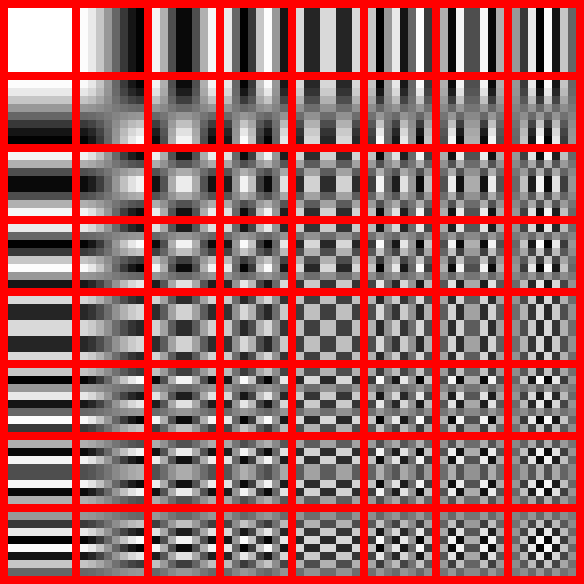
\includegraphics[width = 0.45\textwidth]{img/marco_teorico/Patrones de DCT.png}
            \caption{Patrones de frecuencia para una imagen de 8x8}
            \label{fig:DCT_pattern}
        \end{figure}
    \subsubsection{JPEG}\label{subsubsec: jpeg}
    JPEG es un algoritmo de compresión con la capacidad de disminuir muy significativamente el tamaño de imágenes con pérdidas poco notorias de calidad \cite{jpeg1992}. En general, este algoritmo es bueno en eliminar aquellos elementos que son difíciles de detectar para el ojo humano, privilegiando la luminiscencia por sobre la crominancia cuya detección es menor debido a la concentración de conos y bastones cuya razón es de 6 a 100. Por tanto, la capacidad de reconocer diferencias de brillo y luz es mucho mayor que la de color. Luego los pasos para este algoritmos son:
    
    \subsubsubsection{Conversión del espacio de color}
        En este paso, se cambia el espacio de color desde RGB a YCbCr. Este último se describe como luminescencia, crominancia azul diferenciada y crominancia roja diferenciada. Agrupando de forma efectiva la dimensión perceptiva de los bastones. La fórmula para esta conversión para cada pixel corresponde a:

        \begin{align*}
            \centering
            Y &= 0.299\cdot R + 0.587 \cdot G + 0.114 \cdot B\\
            C_b &= 128 - 0.168736\cdot R - 0.331264 \cdot G + 0.5 \cdot B\\
            C_r &= 128 + 0.5 \cdot R - 0.418688 \cdot G - 0.081312 \cdot B
        \end{align*}

        Esta operación es invertible y no tiene pérdida de información.
        
    \subsubsubsection{Submuestreo de la crominancia}
        En consecuencia de lo mencionado respecto a las características de la visión humana y en el contexto del nuevo espacio de color. Este paso se dedica a submuestrear la información de las imágenes en Cb y Cr a razón de $\frac{1}{4}$ calculando un promedio cada 2x2 pixeles redefiniendo la imagen según estos valores, disminuyendo su tamaño a $\frac{1}{4}$ lo que puede después ser adaptado al tamaño original haciendo upsampling posteriormente para la reconstrucción.
    \subsubsubsection{Transformada de coseno discreta}
        Se aprovecha de la incapacidad del ojo humano para distinguir elementos de alta frecuencia, es decir, aquellos cambios muy rápidos de información entre píxeles para el caso de imágenes. El primer paso corresponde a la división por bloques, en el caso de este algoritmo, son bloques de 8x8 píxeles, cada valor de esta matriz se desplazan del conjunto $[0,256]$ al conjunto $[-128,127]$.\\

        Una vez hecho esto, se genera una matriz de 8x8 donde existen 64 posibles combinaciones de frecuencia según la transformada discreta de coseno en 8x8,es decir, 64 combinaciones base de imágenes de frecuencia. Esta como se mencionó antes es muy útil en términos de concentración de energía. De estas 64 posibilidades se cuenta la cantidad necesaria de cada una para reconstruir la imagen.
    \subsubsubsection{Cuantización}
        Una vez se tiene las repeticiones de frecuencia donde las más altas frecuencias se ubican al extremo derecho. Una matriz de cuantización se aplica, la cual según la calidad de compresión aumentará sus valores de abajo hacia arriba y de derecha a izquierda. A esta división se le busca el entero más cercano, donde naturalmente, aquellas frecuencias altas de menor aparición resultarán nulas y las de menor frecuencia mantendran un valor mayor.
    \subsubsubsection{Longitud de ejecución y codificación Huffman}
        De este resultado, se genera una codificación que recorre toda la imagen de forma serpenteada desde la esquina superior derecha a la inferior izquierda agrupandola en un arreglo. Y con la longitud de ejecución se declara la cantidad de veces que se repite un valor de forma consecutiva en vez de agregarlo esa cantidad de veces.
        

\section{Orden de Morton}\label{sec:morton_order}
    El orden de Morton, también conocido como \textit{Z-order curve}, es una técnica de indexación espacial que permite mapear puntos en un espacio multidimensional (por ejemplo, 2D o 3D) a un valor escalar unidimensional preservando, en la medida de lo posible, la localidad espacial. Fue introducida con el objetivo de mejorar la eficiencia en el acceso secuencial a bases de datos geoespaciales. \cite{morton1966zorder}\\

    La representación tradicional de datos tridimensionales como las nubes de puntos no impone ningún orden explícito sobre los puntos. Sin embargo, muchos algoritmos de compresión, estructuración jerárquica (como octrees) o renderizado acelerado requieren organizar los datos de forma que puntos cercanos en el espacio también estén cercanos en memoria o en disco. El orden de Morton proporciona esta capacidad mediante una codificación binaria de las coordenadas espaciales.
    
    \subsection{Intercalación de bits}
    
    El principio fundamental del orden de Morton es la intercalación de los bits de cada una de las coordenadas espaciales. Dado un punto en el espacio tridimensional con coordenadas enteras \((x, y, z)\), cada coordenada se representa como un entero binario de igual longitud (por ejemplo, 10 bits si el espacio está cuantizado a \(2^{10} = 1024\) unidades por eje).
    
    La clave está en construir un valor escalar \(m\) a partir de los bits de \(x\), \(y\) y \(z\) intercalados de la siguiente manera:
    
    \[
    x = \sum_{i=0}^{b-1} x_i \cdot 2^i, \quad
    y = \sum_{i=0}^{b-1} y_i \cdot 2^i, \quad
    z = \sum_{i=0}^{b-1} z_i \cdot 2^i
    \]
    
    \[
    \Rightarrow \text{Morton code: } 
    m = \sum_{i=0}^{b-1} \left( x_i \cdot 2^{3i} + y_i \cdot 2^{3i + 1} + z_i \cdot 2^{3i + 2} \right)
    \]
    
    En otras palabras, los bits de menor peso de \(x, y, z\) ocupan las posiciones 0, 1, 2 respectivamente en \(m\); los siguientes bits ocupan las posiciones 3, 4, 5; y así sucesivamente. Este procedimiento genera un valor único que se puede utilizar para ordenar o indexar los puntos en memoria.
    
    \subsection{Propiedades}
    
    El orden de Morton tiene las siguientes propiedades fundamentales:
    
    \begin{itemize}
        \item \textbf{Preservación de localidad:} puntos cercanos en el espacio tridimensional tienden a tener códigos Morton similares (aunque no garantiza una vecindad exacta).
        \item \textbf{Jerarquía implícita:} al truncar los bits menos significativos del código Morton, se obtiene una representación de menor resolución del punto, lo que se utiliza en estructuras como octrees.
        \item \textbf{Eficiencia computacional:} la intercalación y desintercalación de bits puede realizarse con operaciones bitwise eficientes, facilitando su implementación en hardware o software optimizado.
    \end{itemize}
    
   En el contexto de esta tesis, el orden de Morton se emplea como mecanismo de indexación para los puntos de la nube durante la partición espacial. Cada punto es convertido a un índice escalar mediante su código Morton, lo que permite realizar una partición espacial coherente en bloques cúbicos jerárquicos, ordenar los puntos para una compresión más eficiente —ya que se agrupan espacialmente en estructuras locales—, y facilitar el acceso jerárquico y progresivo a los datos para tareas como renderizado o reconstrucción. Así, el orden de Morton no solo sirve como herramienta teórica de codificación, sino que actúa como el eje central sobre el cual se organiza la estructura jerárquica de la compresión propuesta.
    
    
    
        

\section{Graph Signal Processing \cite{ortega2022gsp}} \label{sec: gsp}
    \subsection{Notación y conceptos básicos de grafos}

    % Primeramente, cabe destacar la notación recurrente al trabajar con grafos. Dado que estos corresponden a una red interconectada de puntos que pueden representar diversas cosas se define su estructura más elemental de la siguiente manera.

    Se define la estructura más elemental de grafos de la siguiente manera:

    \begin{itemize}
        \item \textbf{Nodos o vértices}: corresponden a los puntos de conexión y pueden representar casi cualquier cosa (puntos en el espacio, puntos en el tiempo, procesos, etc.). Se denotan como $\mathcal{V} = \{v_1,v_2,...,v_n\}$.
        \item \textbf{Aristas}: denotan la conexión entre dos vértices. Pueden ser direccionados o no direccionados. Se denotan como $\mathcal{E} = \{e_1,e_2,...,e_m\}$. A veces se denota como $e_{ij} = v_i v_j$, implicando que es la arista que conecta el nodo $i$ con el nodo $j$. En caso de ser direccionadas, decimos que $e_{ij} \neq e_{ji}$. Para las no direccionadas, se cumple que $e_{ij} = e_{ji}$.
        \item \textbf{Pesos}: los ponderadores asociados a cada arista. Estos valores tienen dos perspectivas: la de \textit{distancia}, donde un mayor valor indica menor conexión, y la de \textit{similitud}, donde un mayor valor indica mayor similitud. Se denota el conjunto de todos los pesos desde un nodo como: $\mathcal{W}_i = \{w_{ij}, \; \forall j \; | \; e_{ij} \in \mathcal{E}_i \}$.
        \item \textbf{Dirección}: como se mencionó, las aristas pueden o no tener un sentido, es decir, la conexión se realiza con una orientación particular de un nodo a otro o no. En este último caso, la relación es totalmente recíproca y equivalente. Esto clasifica a los grafos en dos tipos: \textit{directos}, que implican pesos distintos y/o conexiones no permitidas, e \textit{indirectos}, cuyos pesos son iguales y las conexiones son en ambos sentidos.
    \end{itemize}

    Desde la perspectiva de grafos en el análisis de señales, se entiende que para cada nodo en $\mathcal{V}$ existe un escalar o un conjunto de escalares que representan un valor de señal. Esta señal puede cambiar en el tiempo o ser estática, todo dependerá de la construcción y el significado del grafo. %Naturalmente, si se construye este paradigma de señales en contexto de grafos se deben trasladar e interpretar los conceptos típicos de señales y procesamiento de señales.\\
    
    Cada grafo está estructural y funcionalmente descrito por estructuras algebraicas simples. En primer lugar tendremos la matriz de adyacencia ($A$), que resume las aristas y pesos en una sola matriz con toda la información del grafo. Sea $a_{ij}$ el elemento $i$,$j$ de la matriz de adyacencia:

    \begin{equation*}
        a_{ij} = w_{ij} \quad \quad \forall (i,j) \in \mathcal{E}    
    \end{equation*}

    \vspace{0.4cm}

    Luego, existe la matriz de grado ($D$) que describe el \textit{grado de conectividad} de cada nodo. Esta será una matriz diagonal, donde cada elemento $d_{ii}$ corresponderá a la suma de los pesos de todas las conexiones del nodo $v_i$.

    \vspace{0.4cm}

    \begin{equation*}
        d_{ii} = \sum_{j}a_{ij}
    \end{equation*}

    \vspace{0.4cm}
    
    Con estos dos elementos, podemos resumir el contenido estructural del grafo en la matriz laplaciana ($L$). Esta matriz se construye a partir de la operación simple de la matriz de grado y la matriz de adyacencia.

    \begin{equation*}
        L = D- A
    \end{equation*}
    
    \vspace{0.4cm}
    
    Adicionalmente, los grafos pueden poseer \textit{self-loops}, es decir, conexiones de nodos hacia sí mismos. En general estos elementos tienen un efecto relevante en las transformadas que se explicarán posteriormente. Matemáticamente un \textit{self-loop} se describe como una arista $e_{ii}$ que conecta un nodo sobre si mismo con un peso $w_{ii}$. Para describir el efecto de éste se introduce el laplaciano generalizado:

    \begin{equation*}
        L_g = C + D - A \quad \quad C = diag(a_{11},a_{22},...,a_{nn})
    \end{equation*}

    \vspace{0.4cm}
    
    Describiendo lo anterior, tendremos completamente representada la estructura del grafo en una sola expresión algebraica. A partir de ella, podremos procesar las señales involucrando. %la información de señal con la información impuesta por su estructura.
    
% Transformada 
\subsection{Transformada Gráfica de Fourier}\label{subsec: gft}

    GFT (\textit{graph fourier transform}) es una transformada ortogonal generada a través de los vectores propios ordenados del laplaciano generalizado. Es decir sean $\{ \phi_1, \phi_2, ..., \phi_n \}$ los vectores propios considerando los valores propios $\lambda_1 \leq \lambda_2 \leq ... \leq \lambda_n$ diremos que:

        \begin{equation*}
            U = [\phi_1, \phi_2, ..., \phi_n] \Longrightarrow GFT = U^T
        \end{equation*}

    Lo que representa una transformada sin pérdida de información, es decir, la señal transformada al dominio espectral de grafo puede ser reconstruida completamente. Sea $x$ la señal original de tamaño $(N,1)$ y $\hat{x}$ los coeficientes transformados de tamaño $(N,1)$. Así, la operación realizada por la transformada se ve de la siguiente manera:

        \begin{equation*}
            \hat{x} = U^Tx \quad \quad x = U\hat{x}
        \end{equation*}

    \vspace{0.4cm} 
    
    Esto implica que ambos espacios son ortogonales al igual que la transformada clásica de Fourier, lo que es visible matemáticamente al notar que:
        \begin{equation*}
            U^T U = I
        \end{equation*} 

    \vspace{0.4cm}
    
    Los valores descritos por $\hat{x} = [\hat{x}_1,\hat{x}_2, ..., \hat{x}_n]$ representan los \textbf{coeficientes transformados} y separan la frecuencia de manera similar a como lo haría la transformada de Fourier clásica por componentes de la siguiente manera:

    \begin{equation*}
        \hat{x}_i \cdot \phi_i = f_i \quad \quad x = \sum_{i=1}^N f_i = \sum_{i=1}^N \hat{x}_i \cdot \phi_i 
    \end{equation*}

    Entendiendo esto, podemos hacer reconstrucciones parciales de la señal, perdiendo parte de su información, pero mostrando su comportamiento general y relevante para analizarla e interpretarla. Para toda señal podremos construir un conjunto $M \subset \{1,2,...,N\}$ tal que:

    \begin{equation*}
        x_M = \sum_{i \in M} f_i
    \end{equation*}

    \vspace{0.4cm}

    Para evaluar la información perdida podremos siempre comparar las reconstrucciones con la señal original, para conocer qué tan representativas son las $|M|$ bases. Por ejemplo, se puede hacer un análisis para distintos conjuntos $M$ comparando la señal según la raíz del error cuadrático medio de la reconstrucción:

    \begin{equation*}
        RMSE(x_M, x) = \sqrt{\frac{\sum_{i=1}^N{\left(x_M(i) - x(i)\right)^2}}{N}}
    \end{equation*}

    
\section{Rate-Distorsion Theory}\label{sec: rdt}
    La teoría de tasa distorsión es una de las muchas derivadas de la teoría de Shannon y la codificación de fuentes. El concepto es aprovechar de la mayor manera posible la redundancia de la fuente sujeto a un criterio de fidelidad. En otras palabras, el objetivo de esta teoría es la representación de la fuente con el menor número de bits posibles (tasa) para una dada calidad de reproducción (distorsión) \cite{ortega1998rate}. \\

    Una reflexión previa relevante para estos métodos es que así como las distintas metodologías de compresión pueden diferir mucho en efectividad según el tipo de dato, también pueden diferir entre muestras. Es por tanto otro objetivo de esta teoría aprovechar lo mejor de ambos mundos, primero utilizando la información muestra a muestra para encontrar los mejores parámetros de compresión como también aprovechar la eventual correlación entre muestras subsecuentes. \\

    Otra mención relevante, es que estos métodos solo hacen sentido en un contexto donde exista un escenario de ganancia-pérdida lo que hace matemáticamente relevante un proceso de optimización. En ese sentido, esta teoría es aplicable para métodos de compresión con pérdida de información, donde la pregunta es; cuánta fidelidad de representación se está dispuesto a perder para reducir el almacenamiento necesario para la fuente o sus indicaciones de transmisión.

    \subsection{Métricas de distorsión}
        Ahora, la definición de la métrica de distorsión no es una discusión trivial, en tanto es relevante considerar una combinación de variables cuantitativas y cualitativas. Es decir, es especialmente relevante para datos que dependen de la percepción del consumidor o usuario, en la mayoría de las casos un humano. En resumen, las métricas deben buscar una correlación con el impacto perceptivo del sujeto.\\

        Sin embargo, lo anterior lleva a otra discusión respecto a la generalidad del método, ya que considerar las diferencias individuales de cada sujeto es impracticable. Este objetivo se ha demostrado complejo de resolver, mas a través del conocimiento especializado, por ejemplo en la percepción del color en tanto su resolución biológica (conos y bastones) o el audio según la capacidad humana de escuchar cierto rango de frecuencias.\\

        Mezclando lo anterior con el error mínimo cuadrado, existe una ponderación perceptual conjunta con una métrica cuantitativa para dimensionar la distorsión de los métodos de compresión con pérdida. Un buen ejemplo, observando lo mencionado anteriormente en JPEG es, en el espacio transformado, enfocar el error en la percepción humana enfocandose matemáticamente en el canal de luminiscencia. Por ejemplo, considerando la distorsión como:

        \begin{equation}
            \mathrm{RMSE}(Y, q) = \frac{1}{\sqrt{n}} \left\| Y - q^{-1}(q(Y)) \right\|_2
        \label{eq: rmse_dist}
        \end{equation}
            
    \subsection{Optimización en sistema concreto}
        Si bien existe una discusión teórica sobre cual es el espacio de optimización y el mejor desempeño en tasa distorsión sin restricciones. La presente investigación se centra en la propuesta de un esquema de codificación que limita la optimización a un sistema específico. Este se puede considerar que captura la relevancia estadística y las dependencias asociadas a la fuente, por tanto, el proceso de optimización se centrará en el mejor punto de operación para un esquema ya no abstracto, sino concreto.\\

        Como se mencionó anteriormente en esta sección, considerando el paradigma analizado anteriormente de codificación basado en transformadas, estamos en un esquema bien definido que cumple con los requisitos descritos anteriormente. Desde ese escenario existen multiplicidad de métodos bien estudiados de optimización tasa-distorsión.

        Es relevante mencionar, que lo anterior también incluiría el conocimiento del decodificador, ya que no considerar la información necesaria para la recuperación de la fuente y la calidad de la fuente recuperada, sería miope para el análisis de tasa-distorsión.\\

        Por lo tanto, estaremos en presencia de un espacio de optimización tasa-distorsión discreto para una tipo de entrada específica. Luego el objetivo es: "Dado un entorno de codificación donde el decodificador es completamente definido, optimizar la codificación de una secuencia particular de imagen tal que cumpla algunos objectivos tasa-distorsión"\cite{ortega1998rate}\\

        Para esta tarea, existen dos elementos relevantes a considerar según la aplicación final esperada para la metodología planteada. Primero, está la complejidad, donde será importante diferenciar entre métodos pensados en tiempo real y aquellos que no lo son. En este último caso, la complejidad siempre que los recursos computacionales lo permitan, no está limitada y se pueden realizar multitud de operaciones a diferencia de una propuesta en tiempo real. Segundo, está la definición de la función de costo donde el diseño debe considerar la prioridad, la ponderación y la escala de los elementos a minimizar y como estos afectan el resultado final. Ya que, como se mencionó anteriormente, existe una relevancia de la percepción no es lo mismo optimizar para un resultado local que para un resultado globalmente óptimo.\\

        \subsubsection{Restricciones de almacenamiento posible}
            En distintos contextos, la optimización de nuestro método puede estar restringido por condiciones físicas de almacenamiento o una tasa de referencia a superar. Por ejemplo, el espacio restante en disco puede limitar las elecciones de parámetros del método. Sea $x(i)$ un punto de operación para una secuencia de código $i$ y $R_T$ una restricción general de memoria. Podemos expresar esto tal que:

            \begin{equation}
                \sum_{i=1}^{N} r_{ix(i)} \leq R_T
            \end{equation}

            o de manera local, siendo $r_t$ una restricción de referencia:

            \begin{equation}
                r_{ix(i)} \leq r_t
             \end{equation}
            Además de alguna métrica $f_i$, $f$ que debe ser minimizada local o globalmente respectivamente.\\

            Este consideracón del almacenamiento posible o de restricción de tasa obliga a considerar no tan solo la métrica de distorsión como la discutida en \ref{eq: rmse_dist} sino también la tasa. Para incluir esta restricción el paradigma más clásico y utilizado ampliamente en el contexto de compresión es la optimización Lagrangiana. Básicamente, se introduce un multiplicador de Lagrange $\lambda \geq 0$ y una función de costo de Lagrange tal que:

            \begin{equation}\label{eq: rdo_lagrange}
                J_{g}(\lambda) = d_{ij} + \lambda \cdot r_{ij}
            \end{equation}

            Donde $d_{ij}$ corresponde a la distorsión para el índice de cuantización $j$ (cierto paso de cuantización) y $r_{ij}$ corresponde a la tasa o tamaño del código que representa dicha información cuantizada. Con esto podemos controlar la relevancia que damos a la tasa en el proceso de optimización minimizando local o globalmente la función objetivo. \\

            Finalmente, hay una cuestión relevante que surge de este análisis respecto a como obtenemos métricas precisas para optimizar resultados en un proceso que no es determinístico. Por ejemplo, al ocupar codificación entrópica, este es un método estadístico y probabilístico que no es independiente de la distribución de los coeficientes transformados. Es por tanto recurrente la utilización de aproximaciones de la tasa, basadas en la compresión específica de la codificación a utilizar y esto es algo que se debe abordar al desarrollar un método de compresión.



\chapter{Estado del Arte}

\section{Codificación por Octree}

La codificación por octree es una técnica jerárquica para representar objetos espaciales que aprovecha la coherencia espacial presente en la mayoría de las nubes de puntos y objetos tridimensionales \cite{meagher1982geometric,loop2016microsoft}. Esta técnica organiza la información en una estructura arbórea en la que cada nodo representa un cubo disjunto en el espacio, cuyo tamaño decrece exponencialmente a medida que se desciende por los niveles del árbol. De esta forma, cada nodo corresponde a una región del universo y se le asigna una propiedad que describe dicha región.\\

Si un nodo describe completamente su región —por ejemplo, si el cubo está completamente vacío o completamente ocupado— se considera un nodo terminal o hoja. En caso contrario, existe una ambigüedad que se resuelve dividiendo la región en ocho subregiones o octantes, que corresponden a los nodos hijos del nodo padre. Esta subdivisión recursiva permite representar objetos con un grado de detalle variable, adaptando la precisión espacial a la complejidad local de la nube de puntos \cite{meagher1982geometric}.\\

\begin{figure}
    \centering
    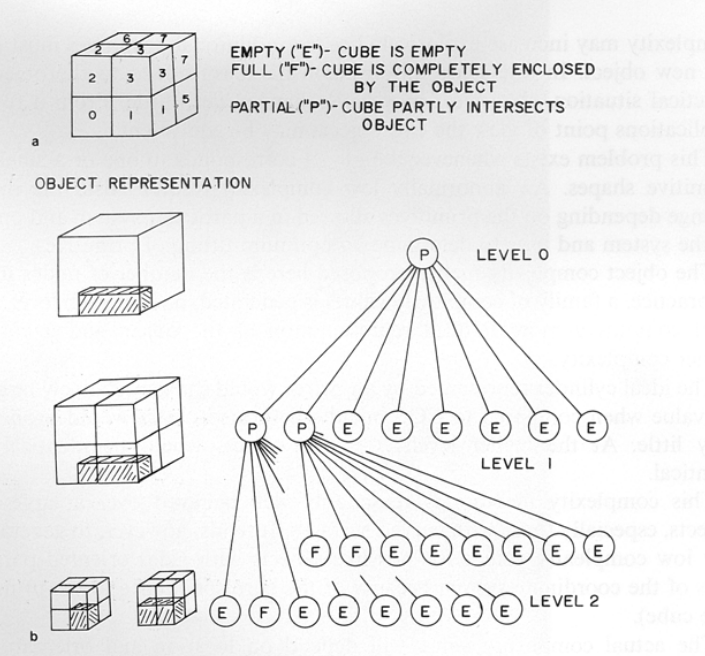
\includegraphics[width=0.5\linewidth]{img/estado_del_arte/octree.png}
    \caption{Representación simple del formato de la codificación por Octree}
    \label{fig:octree}
\end{figure}

Una ventaja esencial de esta estructura es que utiliza una única forma primitiva, el cubo, lo que simplifica tanto el almacenamiento como las operaciones sobre los datos. Además, al representar el objeto a múltiples niveles de resolución, el octree permite gestionar la memoria de manera eficiente, almacenando los detalles más finos sólo cuando es necesario y manteniendo un nivel más grueso cuando el detalle no es crítico. Esto facilita también realizar operaciones espaciales como la detección de colisiones, la visualización con ocultación y operaciones booleanas de forma eficiente, ya que el recorrido jerárquico permite acceder a las regiones del espacio de manera ordenada, evitando búsquedas exhaustivas \cite{meagher1982geometric}.\\

Asimismo, la estructura jerárquica del octree permite que muchas operaciones puedan ser detenidas en niveles superiores cuando la precisión requerida se ha alcanzado, lo que reduce significativamente el costo computacional. Por otro lado, la naturaleza dividida del árbol, donde cada nodo genera hasta ocho subcálculos independientes, hace que el procesamiento pueda ser paralelizado fácilmente, mejorando la velocidad en sistemas con múltiples procesadores.\\

En cuanto a la representación, cada nodo en el octree está identificado por una dirección única que indica su posición espacial relativa al nodo raíz y su nivel dentro de la jerarquía. Las propiedades asignadas a los nodos pueden ir desde una simple clasificación en estados como vacío, parcialmente lleno o completamente lleno, hasta incluir atributos complejos como tipo de material, color o densidad, ampliando así la riqueza de la representación \cite{loop2016microsoft}.\\

Aunque la codificación por octree puede requerir un mayor consumo de memoria, generalmente proporcional al área superficial del objeto representado, su capacidad para modelar la estructura espacial de la nube de puntos de manera compacta y adaptativa la convierte en una herramienta esencial para la compresión y manipulación eficiente de datos tridimensionales \cite{meagher1982geometric}. Así, el codificado por octree abre la posibilidad de aprovechar la correlación espacial inherente a las nubes de puntos, permitiendo una representación estructuralmente coherente y eficiente que facilita tanto el almacenamiento como el procesamiento posterior \cite{loop2016microsoft}.

\section{Run Length Golomb-Rice Entropy Coder}\label{sec: rlgr}

El codificador de entropía Run Length Golomb-Rice (RL-GR) es un método efectivo y de baja complejidad para la compresión sin pérdida de secuencias binarias con estructuras de tipo \textit{run-length}, es decir, secuencias con repeticiones consecutivas del mismo símbolo \cite{malvar2006adaptive,sayood2006introduction}. Combinando codificación por longitud de carrera (Run Length) con codificación Golomb-Rice, este método permite representar eficientemente tanto secuencias de ceros prolongadas como valores pequeños comunes en señales residuales.

La codificación Golomb-Rice es un caso particular de codificación de Golomb donde el parámetro divisor es una potencia de dos, lo que permite una implementación computacionalmente eficiente \cite{malvar2006adaptive}. Este codificador es ampliamente utilizado en estándares de compresión como MPEG y JPEG-LS \cite{jpeg1992}, debido a su equilibrio entre rendimiento y simplicidad. En el contexto de nubes de puntos, RL-GR se emplea para comprimir mapas de ocupación, residuos de predicción o secuencias binarias derivadas del escaneo espacial jerárquico, donde los datos presentan redundancia local y patrones repetitivos.

\section{\textit{Learning separable transforms by inverse covariance estimation}} \label{sec: lst_ice}

Este trabajo presenta un enfoque para diseñar transformadas adaptativas que se ajusten automáticamente a las características específicas de los datos de entrada. La idea principal es que en lugar de usar transformadas fijas como DCT o DST, se pueden crear transformadas que cambien según las propiedades estadísticas de la señal a procesar.\\

El aporte más relevante son las Transformadas Trigonométricas Discretas Paramétricas (p-DTTs), que se basan en la representación de la señal como un grafo de línea. Un grafo de línea es simplemente una cadena de nodos conectados secuencialmente, donde cada nodo representa un píxel o muestra de la señal. La innovación clave consiste en agregar conexiones adicionales llamadas \textit{self-loops} en los extremos de esta cadena, lo que modifica las propiedades de la transformada resultante.\\

Matemáticamente, las p-DTTs se definen mediante dos parámetros $(\alpha, \beta)$ que controlan el peso de estos \textit{self-loops} en el primer y último nodo del grafo respectivamente. Cuando $\alpha = \beta = 0$, se obtiene la transformada DCT-2 clásica. Variando estos parámetros se pueden generar otras transformadas conocidas como DST-4 o DST-7, pero también crear nuevas transformadas adaptadas a características específicas del contenido modificando el laplaciano.\\

\begin{equation}
    L(\alpha, \beta) = \text{diag}(\alpha, 0, \ldots, 0, \beta) + L_{DCT}
= \begin{bmatrix}
\alpha & 0 & \cdots & 0 & 0 \\
0 & 0 & \cdots & 0 & 0 \\
\vdots & \vdots & \ddots & \vdots & \vdots \\
0 & 0 & \cdots & 0 & 0 \\
0 & 0 & \cdots & 0 & \beta
\end{bmatrix} + \begin{bmatrix}
1 & -1 & 0 & \cdots & 0 \\
-1 & 2 & -1 & \cdots & 0 \\
0 & -1 & 2 & \cdots & 0 \\
\vdots & \vdots & \ddots & \ddots & \vdots \\
0 & 0 & \cdots & -1 & 1
\end{bmatrix}
\end{equation}


Ocupando esta metodología se pueden replicar un conjunto preciso de transformadas paramétricas demostrando la capacidad de adaptar dinámicamente las transformadas gráficas. Aplicando distintos valores, se pueden obtener según la dinámica de la señal a procesar un conjunto de señales, según la siguiente tabla:

\begin{table}[H]
    \centering
    \caption{Relación entre parámetros $\alpha$ y $\beta$ con las transformadas seleccionadas}
    \begin{tabular}{c|ccc}
    \toprule
    $\alpha \backslash \beta$ & 0 & 1 & 2 \\
    \midrule
    0 & DCT-2 & DCT-8 & DCT-4 \\
    1 & DST-7 & DST-1 & DST-5 \\
    2 & DST-4 & DST-6 & DST-2 \\
    \bottomrule
    \end{tabular}
\end{table}

La relevancia de este enfoque para nubes de puntos radica en que demuestra cómo la modificación estructural de un grafo mediante \textit{self-loops} puede mejorar significativamente el rendimiento de las transformadas. Mientras que las p-DTTs operan sobre grafos de línea simples para señales 2D, el principio subyacente de adaptar la estructura del grafo según las características locales de la señal puede extenderse a grafos 3D más complejos para el procesamiento de atributos de color en nubes de puntos.

\section{\textit{Point Cloud Attribute Compression With Graph Transform}}\label{sec: pcac_geometric}

La compresión de atributos de nubes de puntos mediante transformada de grafos es una técnica avanzada que explota la estructura irregular de los datos tridimensionales \cite{zhang2014point,pavez2020region}. A diferencia de los métodos clásicos que utilizan DCT o \textit{wavelets}, la transformada de grafos permite modelar relaciones entre puntos a través de un grafo, donde los nodos representan puntos y las aristas modelan su proximidad o conectividad.\\

La transformada de Fourier sobre grafos (GFT) permite descomponer los atributos, como el color o la reflectancia, en una base adaptada a la estructura del grafo, capturando mejor la correlación espacial entre puntos \cite{ortega2022gsp}. De esta forma, la energía de los atributos tiende a concentrarse en unos pocos coeficientes de baja frecuencia, lo que permite una compresión más efectiva.\\

Considerando que la información geométrica ya ha sido codificada mediante métodos como los mencionados anteriormente en la sección de codificación por octree, se asume que la información estructural ya la posee el decodificador y por tanto la compresión de los atributos puede utilizar esta información sin necesitar agregar instrucciones mayores respecto a la información estructural \cite{loop2016microsoft}.\\

Luego, este método construye un grafo basándose en distancias discretas de puntos voxelizados donde las conexiones existirán siempre que dicha distancia no supere cierto umbral. Estos pesos o valores de arista son inversamente proporcionales y tienen la diagonal cúbica como límite describiéndose de la siguiente manera:

\begin{equation}
    w_1 = 1, \quad w_2 = \frac{1}{\sqrt{2}}, \quad w_3 = \frac{1}{\sqrt{3}}
\end{equation}

Lo que describirá una matriz de adyacencia simétrica de la forma:
\[
A = 
\begin{bmatrix}
0   & w_3 & w_2 & 0   & 0   & 0 \\
w_3 & 0   & w_1 & w_3 & 0   & 0 \\
w_2 & w_1 & 0   & w_2 & 0   & 0 \\
0   & w_3 & w_2 & 0   & w_1 & w_2 \\
0   & 0   & 0   & w_1 & 0   & w_1 \\
0   & 0   & 0   & w_2 & w_1 & 0
\end{bmatrix}
\tag{5}
\]

Ocupando esta construcción de grafo, se procede a hacer el proceso de transformada gráfica descrita en el marco teórico \cite{ortega2022gsp}. Este entregará un laplaciano que se asegura es una matriz semidefinida positiva. Luego, entendiendo que la transformada gráfica contiene solo información disponible en el decodificador, el mensaje se convierte en la codificación de los coeficientes de las bases posterior a su cuantificación.\\

Al ser este un enfoque nuevo para su época, la comparación se hace respecto a la DCT de una dimensión para el encadenamiento de todos los bloques. Sean el nivel 5 bloques de 16x16x16, el nivel 6 bloques de 8x8x8, el nivel 7 bloques de 4x4x4 y el nivel 8 bloques de 2x2x2, se muestran los siguientes resultados en la siguiente figura:

\begin{figure}
    \centering
    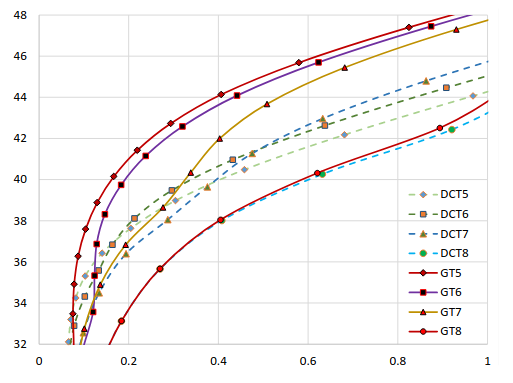
\includegraphics[width=0.5\linewidth]{img/estado_del_arte/block_GFT.png}
    \caption{Rendimiento de compresión (en dB) frente a la tasa de bits (en bpv) para el codificador propuesto utilizando una Transformada de Grafos y DCT para los niveles de octree 5, 6, 7 y 8 (correspondientes a tamaños de cubo de 16, 8, 4 y 2, respectivamente) \cite{zhang2014point}}
    \label{fig:block_gft}
\end{figure}

Los datos utilizados provienen de nubes de puntos 3D generadas en tiempo real

\chapter{Metodología}
% Compactación de la energía será relevante mencionar en marco teórico
El diseño de este trabajo se basa en la implementación novedosa de los conceptos descritos anteriormente en el marco teórico. Como la mayoría de los esquemas de compresión, la propuesta aquí descrita implementa modificaciones sobre un desarrollo base que pretenden mejorar los resultados de compresión integrando nuevas metodologías para privilegiar la compactación de la energía de aquellos elementos más informativos de la señal.

\section{Esquema de compresión}
    Privilegiando la comprensión del lector, los siguientes diagramas muestran de forma general las etapas del esquema de compresión. El primero muestra el flujo de los datos geométricos y dónde precisamente en el esquema completo de compresión está ubicado el algoritmo propuesto. El segundo muestra el esquema de compresión propuesto con las etapas utilizadas para el presente trabajo, las cuales se ahondarán durante este capítulo.

    \begin{figure}
        \centering
        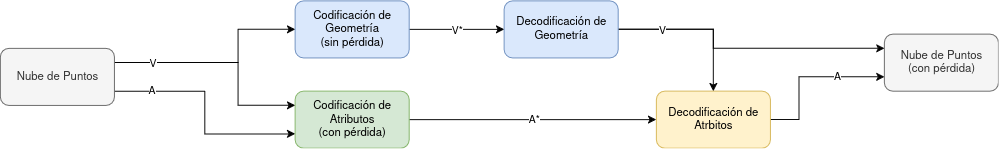
\includegraphics[width=1\textwidth]{img/metodología/Full-Scheme.png}
        \caption{Esquema completo de compresión}
        \label{fig:enter-label}
    \end{figure}

    En la figura anterior, se muestra la geometría de la nube de puntos conocida y sin pérdida tanto por el codificador como por el decodificador de atributos. Lo anterior es fundamental, pues permite a la implementación asumir la geometría como conocida y, por tanto, la utiliza sin agregar información adicional al flujo de bits. Entendiendo esto, la siguiente figura muestra el esquema de codificación propuesto para los atributos de color de la nube de puntos.

    \begin{figure}
        \centering
        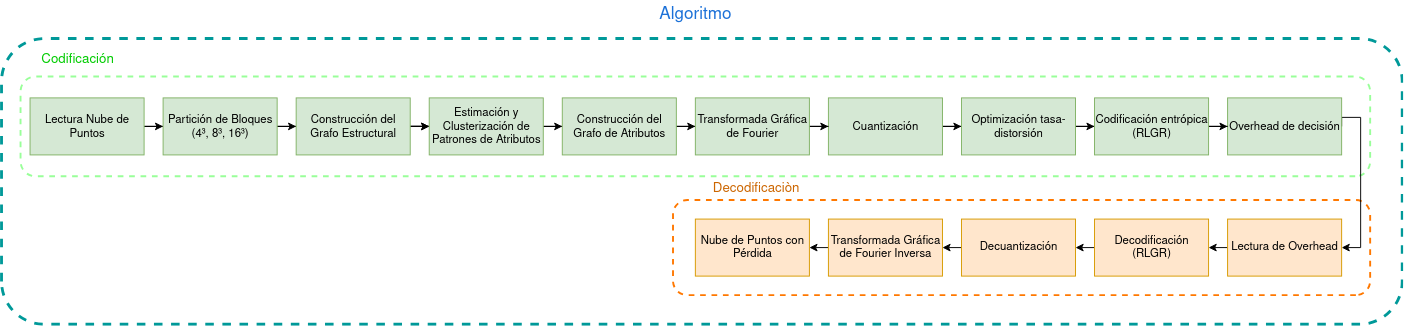
\includegraphics[width=1\textwidth]{img/metodología/PCADC_Algorithm_Hor.png}
        \caption{Esquema algoritmo compresión de atributos}
        \label{fig:enter-label}
    \end{figure}

\section{Datos Utilizados}
% - Describir el dataset utilizado (nombre, resolución, fuente, etc.)
    Lo primero a mencionar son las características de los datos utilizados para la evaluación de la metodología que se describirá a continuación, en tanto que esto condiciona el procesamiento en su posterioridad. \\

    Existen distintas formas de obtener datos de nubes de puntos, que limitan la resolución y caracterizan los datos en tanto su cantidad máxima de puntos y las referencias espaciales máximas que se pueden representar. En este trabajo se utilizaron dos bases de datos clásicas y ampliamente estudiadas en el campo de compresión de nubes de puntos.\\

    De forma general, ambas fuentes de datos contienen nubes de puntos descritas de la misma manera con metodologías de obtención distintas lo que implica ciertas diferencias de su contenido lo que condiciona el análisis posterior. Sin embargo la representación es la misma y consiste en un conjunto de puntos espacialmente ubicados según ejes cartesianos ($x$, $y$, $z$) restringidos por una grilla rectangular en 3D que sin pérdida de generalidad se asumen pertenecientes a un enmallado de números enteros.\cite{deon2017voxelized} Se dice de manera formal, que cada uno de estos puntos cartesianos se ubica en la grilla a través de un \textit{voxel}, que sería el equivalente a un pixel para un objeto tridimensional. En este contexto, se habla de que ambas fuentes de datos, poseen nubes de puntos voxelizadas cuya cantidad de puntos es no homogenea. Es importante destacar además que los \textit{voxeles} pueden estar tanto ocupados como desocupados, a diferencia de una imagen que posee información de color y señal en cada uno de sus píxeles, lo que justifica la búsqueda de estructuras no convencionales para la representación de la señal.\\
    
    \subsection{\textit{8i Voxelized Full Bodies}}
        Para este primer caso, principal caso de análisis por su complejidad y diversidad de fuentes, se trata de cuatro secuencias dinámicas de un sujeto en movimiento ocupando distintas vestimentas. Las secuencias están tipificadas como \textit{Long Dress}, \textit{Loot}, \textit{Red and Black} y \textit{Soldier} cada una capturada de treinta frames por segundo en un periodo de diez segundos, lo que considera aproximadamente 300 imágenes por secuencia.

        \begin{figure}[H]
            \centering
            \begin{subfigure}[b]{0.22\linewidth}
                \centering
                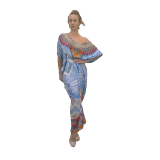
\includegraphics[width=\linewidth]{img/metodología/longdress_thumb.png}
                \caption{Longdress}
                \label{fig:longdress}
            \end{subfigure}
            \begin{subfigure}[b]{0.22\linewidth}
                \centering
                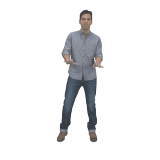
\includegraphics[width=\linewidth]{img/metodología/loot_thumb.png}
                \caption{Loot}
                \label{fig:loot}
            \end{subfigure}
            \begin{subfigure}[b]{0.22\linewidth}
                \centering
                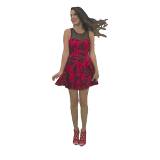
\includegraphics[width=\linewidth]{img/metodología/redandblack_thumb.png}
                \caption{Red and Black}
                \label{fig:redandblack}
            \end{subfigure}
            \begin{subfigure}[b]{0.22\linewidth}
                \centering
                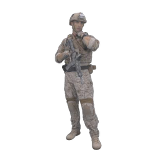
\includegraphics[width=\linewidth]{img/metodología/soldier_thumb.png}
                \caption{Soldier}
                \label{fig:soldier}
            \end{subfigure}
            \caption{Ejemplos Base de Datos - 8iVFB v2.}
            \label{fig:datasets}
        \end{figure}

        Estos datos fueron obtenidos a través de cuarenta y dos cámaras RGB configuradas en catorce agrupaciones donde cada uno de estas, actua logicamente como una cámara de cuatro canales incluyendo la reflectancia. Se ocupa la misma resolución espacial para cada una de las secuencias: un cubo de profundidad diez, es decir, una grilla de $2^{10} = 1024$ posiciones por orientación, entregando un total de $2^{10^{3}} \approx 1.07e9$ posibles posiciones. De todas maneras, para cada secuencia el cubo es escalado para ser el cubo delimitador más pequeño posible que contenga la secuencia. Es importante destacar que como típicamente la altura del sujeto es la dimensión más grande de la secuencia, la proporcionalidad en sistema internacional de los vóxeles estará dada por la siguiente expresión: 
        \begin{equation}
         \text{proporción} \frac{[m]}{[voxel]} \approx \frac{\text{altura}\;[m]}{1024 \; [voxels]}
        \end{equation}

        Para generar cierto tipo de intuición, para un sujeto de $1.8$ metros tendremos aproximadamente $1.75$ milímetros por voxel. Lo que implica que son objetos pensados para percibir a distancia.\\
        % - Justificar la elección del conjunto de datos
        Luego, la relevancia de este conjunto está principalmente en la diversidad de color, una mayor continuidad y la compresión en contexto de cuerpo completo.

    \subsection{\textit{Microsoft Voxelized Upper Bodies}}
        Este conjunto de datos a diferencia del anterior, consiste en imágenes de los troncos superiores de cinco sujetos catalogados como: \textit{Andres}, \textit{David}, \textit{Phil}, \textit{Ricardo} y \textit{Sara}. Cada uno de estos sujetos son capturados en siete y diez segundos completando dos secuencias. Las secuencias más cortas están capturadas con profundidad nueve, es decir, una grilla de $2^{9^{3}}$, mientras las más largas con una profundidad de diez.\\
        La obtención de estos datos se hizo mediante cuatro cámaras RGBD a treinta cuadros por segundo entregando un total de 210 y 300 imágenes para cada versión respectiva. Como es razonable, la profundidad cambia la resolución de la nube de puntos donde aproximadamente los voxeles de profundidad nueve corresponden a $1.5\;[mm]$ cúbicos mientras que las de profundidad diez corresponden a $0.75\;[mm]$ cúbicos. \cite{loop2016microsoft} 

        \begin{figure}[H]
            \centering
            \begin{subfigure}[b]{0.19\linewidth}
                \centering
                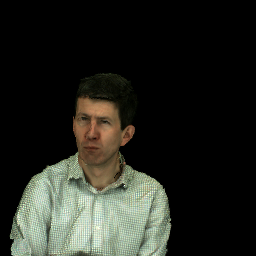
\includegraphics[width=\linewidth]{img/metodología/andrew_thumb.png}
                \caption{Andrew}
                \label{fig:andrew}
            \end{subfigure}
            \begin{subfigure}[b]{0.19\linewidth}
                \centering
                
\includegraphics[width=\linewidth]{img/metodología/david_thumb.png}
                \caption{David}
                \label{fig:david}
            \end{subfigure}
            \begin{subfigure}[b]{0.19\linewidth}
                \centering
                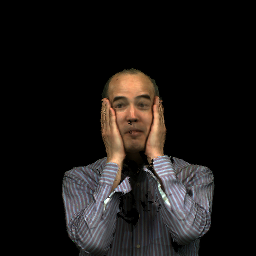
\includegraphics[width=\linewidth]{img/metodología/phil_thumb.png}
                \caption{Phil}
                \label{fig:phil}
            \end{subfigure}
            \begin{subfigure}[b]{0.19\linewidth}
                \centering
                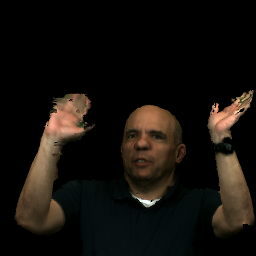
\includegraphics[width=\linewidth]{img/metodología/ricardo_thumb.png}
                \caption{Ricardo}
                \label{fig:ricardo}
            \end{subfigure}
            \begin{subfigure}[b]{0.19\linewidth}
                \centering
                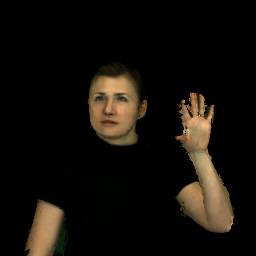
\includegraphics[width=\linewidth]{img/metodología/sarah_thumb.png}
                \caption{Sarah}
                \label{fig:sarah}
            \end{subfigure}
            \caption{Ejemplos Base de Datos - MVUB.}
            \label{fig:seq_immersive}
        \end{figure}
        % - Justificar la elección del conjunto de datos
        En este caso, este conjunto se caracteriza entonces por una resolución más fina y es relevante para observar el desempeño del algoritmo a corta distancia. Para análisis cualitativos será fundamental observar como se diferencia el desempeño del método entre este conjunto de datos y el anterior. 

    Finalmente es importante mencionar que ambas bases de datos presentan las nubes de puntos indexadas según el orden de Morton explicado en el marco teórico. Este orden privilegia la cercanía indexada de aquellos puntos que poseen mayor cercanía representándolos como una lista unidimensional.
    
\section{Partición de la Nube de Puntos}
    % - Explicar el proceso de división en bloques (por ejemplo, tamaños 4³, 8³, 16³)
    % - Justificar la necesidad de particionar
    % - Relación con la adaptabilidad local del método
    De la misma forma que los métodos clásicos implementan el paradigma de divide y vencerás para los problemas computacionales, la compresión de nubes de puntos tiene como primer paso la división por bloques. Lo que sería tradicionalmente una división de una imagen en ventanas de cierta cantidad de pixeles, aquí se divide el espacio en cubos de cierta cantidad de vóxeles.\\

    En este contexto, lo primero es mencionar que los tamaños de bloques deben ser potencias de dos, ya que como se mencionó en la sección anterior, la profundidad de resolución se corresponde con potencias binarias. Por lo tanto la siguiente expresión limita la posibilidad de tamaños de bloques según lo siguiente:

    \begin{equation}
        b = 2^k, \quad k \in \mathcal{N}
    \end{equation}

    Luego, se operan las coordenadas según dicho tamaño de bloque con el objetivo de determinar como los puntos se ubican dentro de estas nuevas celdas tridimensionales. Matemáticamente se hace una cuantización escalar la cuál nos entrega la frontera más cercana para los bloques del tamaño elegido. Sea $v_i$ la posición del punto para el índice $i$.

     \begin{equation}
         v^{block}_i = \left\lfloor \frac{v_i}{b} \right\rfloor \cdot b
     \end{equation}

     De esta manera, se mapea cada punto al origen del bloque cúbico al que pertenece. Por ejemplo, si $b=8$, un punto $(13,7,19)$ se mapea a $(0, 8,16)$ indicando la pertenencia al bloque de dicho origen. Luego, es fácil observar que si a estos puntos cuantizados les calculamos sus diferencias podemos encontrar aquellos donde existen cambios de bloques, identificando precisamente la pertenencia de cada punto. Matemáticamente describimos la siguiente métrica:

     \begin{equation}
         \Delta _i = || v^{block}_{i+1} - v^{block}_i ||_1
     \end{equation}

     Donde, encontraremos los puntos que pertenecen a cierto bloque siempre y cuando $\Delta_i = 0$ para las distintas comparaciones entre puntos. Esto nos entregará un conjunto de índices, que gracias al orden de Morton, son secuenciales y por tanto se representan por su índice inicial y final.\\

     A modo de ejemplo, la siguiente figura muestra el primer bloque de la secuencia \textit{Long Dress} para un tamaño de bloque de dieciséis.
     \begin{figure}
         \centering
         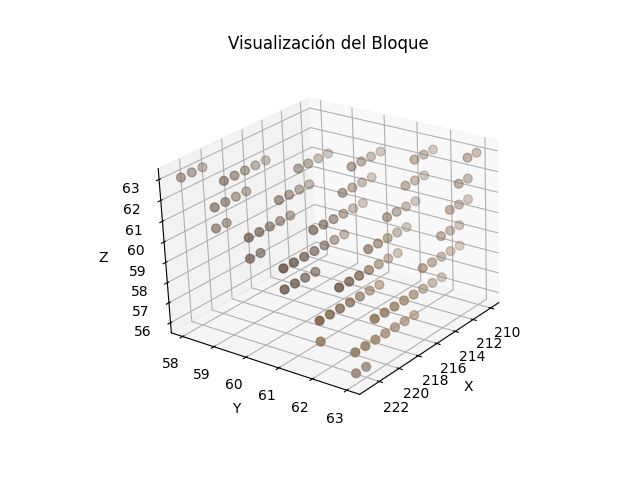
\includegraphics[width=0.8\linewidth]{img/metodología/Bloque_Ejemplo.png}
         \caption{Ejemplo de Bloque ($b=16$)}
         \label{fig:enter-label}
     \end{figure}les.\\

    En este contexto, lo primero es mencionar que los tamaños de bloques deben ser potencias de dos, ya que como se mencionó en la sección anterior, la profundidad de resolución se corresponde con potencias binarias. Por lo tanto la siguiente expresión limita la posibilidad de tamaños de bloques según lo siguiente:

    \begin{equation}
        b = 2^k, \quad k \in \mathcal{N}
    \end{equation}

    Luego, se operan las coordenadas según dicho tamaño de bloque con el objetivo de determinar como los puntos se ubican dentro de estas nuevas celdas tridimensionales. Matemáticamente se hace una cuantización escalar la cuál nos entrega la frontera más cercana para los bloques del tamaño elegido. Sea $v_i$ la posición del punto para el índice $i$.

     \begin{equation}
         v^{block}_i = \left\lfloor \frac{v_i}{b} \right\rfloor \cdot b
     \end{equation}

     De esta manera, se mapea cada punto al origen del bloque cúbico al que pertenece. Por ejemplo, si $b=8$, un punto $(13,7,19)$ se mapea a $(0, 8,16)$ indicando la pertenencia al bloque de dicho origen. Luego, es fácil observar que si a estos puntos cuantizados les calculamos sus diferencias podemos encontrar aquellos donde existen cambios de bloques, identificando precisamente la pertenencia de cada punto. Matemáticamente describimos la siguiente métrica:

     \begin{equation}
         \Delta _i = || v^{block}_{i+1} - v^{block}_i ||_1
     \end{equation}

     Donde, encontraremos los puntos que pertenecen a cierto bloque siempre y cuando $\Delta_i = 0$ para las distintas comparaciones entre puntos. Esto nos entregará un conjunto de índices, que gracias al orden de Morton, son secuenciales y por tanto se representan por su índice inicial y final.\\

     A modo de ejemplo, la siguiente figura muestra el primer bloque de la secuencia \textit{Long Dress} para un tamaño de bloque de dieciséis.
     \begin{figure}
         \centering
         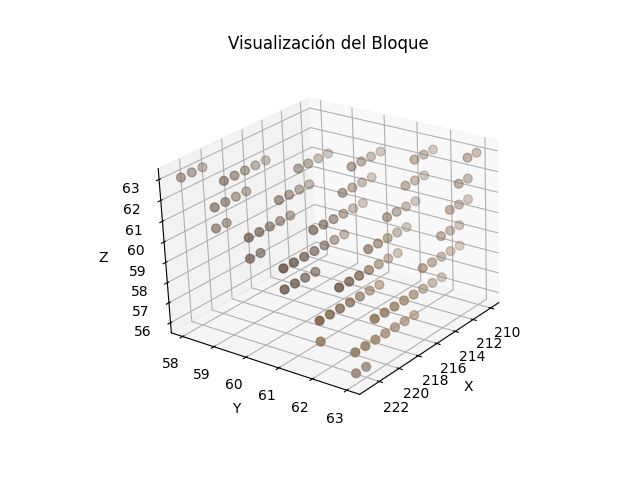
\includegraphics[width=0.8\linewidth]{img/metodología/Bloque_Ejemplo.png}
         \caption{Ejemplo de Bloque ($b=16$)}
         \label{fig:enter-label}
     \end{figure}
    
    % DAR UN EJEMPLO??? + Visual
\section{Construcción del Grafo Estructural}
% - Explicar cómo se conecta cada punto con sus vecinos
% - Tipo de conectividad usada (k-NN, radio, etc.)
% - Qué representa el grafo: estructura geométrica de la nube
    La implementación del método se basa fuertemente en la interacción de las muestras de forma local respecto a su vecindad. Pero ninguno de estos conceptos hace sentido sin una estructura subyacente a la cuál se le pueda entregar esta interpretación. Por otro lado, como se mencionó en la primera sección de este capítulo, el desarrollo está sustentado bajo la hipótesis de que tanto el codificador como el decodificador están en pleno conocimiento de la geometría de la nube. Con esto en mente entonces, es relevante para el método propuesto aprovechar al máximo la información espacial para la compresión para evitar la necesidad de información adicional.\\

    Considerando lo anterior, el primer paso es construir el grafo estructural por bloque, esto está definido de la misma manera que se mencionó en la sección \ref{sec: pcac_geometric}. Esta será la estructura adyacente, donde lo importante a notar que la relación de los nodos están dados por la diagonal cúbica unitaria y los pesos serán inversamente proporcionales a dicha distancia.\\

    Finalmente, es importante notar que cada nodo puede tener una multiplicidad de vecinos no homogénea, lo que diferencia esta estructura a lo que sería el paradigma clásico de imágenes. Lo anterior implica que este grafo puede tomar muchas formas y cada nodo posee una cantidad distinta de vecinos, para ilustrar esto se presenta la siguiente figura:

    \begin{figure}
        \centering
        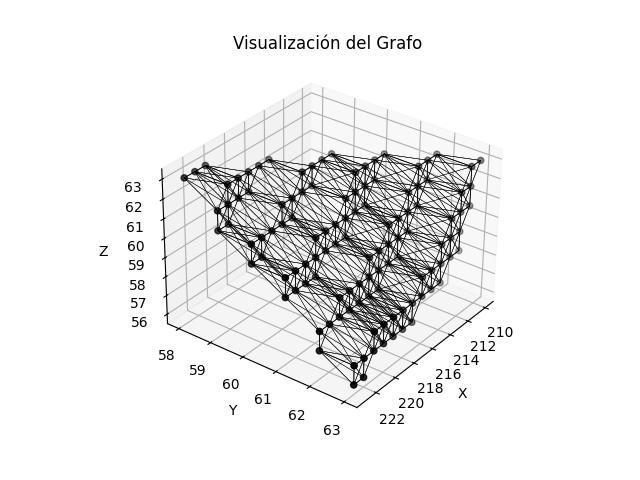
\includegraphics[width=0.85\linewidth]{img/metodología/Grafo_Ejemplo.png}
        \caption{Ejemplo de Grafo ($b=16$)}
        \label{fig:enter-label}
    \end{figure}
    % SERÁ NECESARIO DECIR ALGO MÁS??? O desarrollar mejor el estado del arte


\section{Análisis de Patrones de Atributos}
    % AUN EN DESARROLLO
    Hasta ahora, toda la metodología ha trabajado con los datos espaciales de la nube de puntos. Sin embargo, el objetivo radica en la compresión de los atributos, lo que podría llamarse los valores de la señal. Atacando lo anterior y usando la lógica heredada de métodos clásicos de codificación basado en transformadas (\ref{sec:transform_based_coding}).\\

    La presente implementación se enfoca en atributos de color RGB, por tanto, el primer paso intuitivo es hacer la transformación que cualitativamente es más informativa descrita por el algoritmo JPEG. En otras palabras, se transforma el espacio de color RGB al espacio YUV sin pérdida de información. Luego, como se mencionó en la sección \ref{subsubsec: jpeg} lo más relevante será privilegiar la información en el canal de luminancia al ser esta para la cual el ojo humano posee mayor resolución.\\

    El presente método de compresión tiene como objetivo declarado ocupar la información de los atributos para establecer un método dependiente de compresión adaptando la estructura del grafo. No obstante, es impracticable la transmisión de los atributos para su utilización tanto así como las decisiones crudas derivadas de ello. Lo anterior, motiva el dilema de transmitir una representación óptima de la información necesaria o de las decisiones tomadas. Optando por lo primero, el objetivo de esta sección es mostrar una estrategia para transmitir representaciones aproximadas de la información de los atributos con un conjunto de bases limitadas.\\

    Por supuesto, para poder lograr esto se hace indispensable la normalización de los bloques para que las representaciones sean atribuibles y clusterizables entre todas. Por tanto, el primer paso es la normalización posicional y rotacional del bloque.

    \subsection{Normalización Espacial}
        Lo primero es centrar los puntos del bloque para elaborar referencias de bloques uniformes. Esta operación es simple y consiste en remover la media por componente al conjunto de puntos del bloque:

        \begin{equation}
            V_i^{c} = V_{i} - \bar{V_i}
        \end{equation}

        Posterior a esto, es relevante orientar todos los bloques en los ejes virtuales donde su variación es máxima. El objetivo de aquellos es que aquellos bloques que representen distribuciones espaciales similares tengan una expresión similar. Para aquellos lo primero es definir la matriz de covarianza del bloque que expresa matemáticamente la variación de cada componente sobre si mismo y entre ellos:

        \begin{equation}
            \mathbf{\Sigma} =
                \begin{bmatrix}
                \mathrm{Var}[x] & \mathrm{Cov}[x,y] & \mathrm{Cov}[x,z] \\
                \mathrm{Cov}[y,x] & \mathrm{Var}[y] & \mathrm{Cov}[y,z] \\
                \mathrm{Cov}[z,x] & \mathrm{Cov}[z,y] & \mathrm{Var}[z]
                \end{bmatrix}
        \end{equation}

        A partir de aquello, podemos encontrar las bases ortogonales que representan la mayor variación del bloque. Para aquello hacemos la descomposición en vectores propios:

        \begin{equation}
            \mathbf{\Sigma} = \mathbf{Q} \mathbf{\Lambda} \mathbf{Q}^\top
        \end{equation}

        Si bien estos vectores propios poseen la rotación en el sentido específicado. Existe la posibilidad de que la rotación genere un efecto espejo, perdiendo la uniformidad de la transformación para todos los bloques. En este sentido, forzamos que el tercer vector propio cumpla con la regla de la mano derecha, o más formalmente que la orientación de la base ortonormal sea positiva.

        \begin{equation}
            \mathbf{q}_3 = \mathbf{q}_1 \times \mathbf{q}_2
        \end{equation}
        
        Con estas bases canónicas rotamos el bloque en las direcciones especificadas normalizando su orientación.
        \begin{equation}
            V^{r}_i = V^{c}_i \mathcal{}{Q}
        \end{equation}

        En el ejemplo presentado en las secciones anteriores, esto se vería de la siguiente forma:

        \begin{figure}
            \centering
            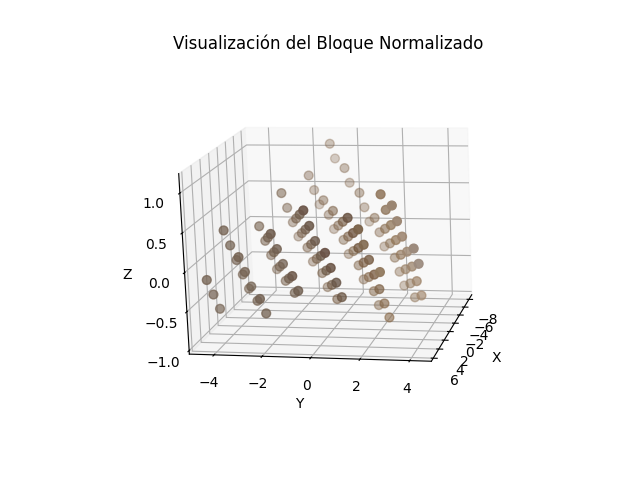
\includegraphics[width=0.85\textwidth]{img/metodología/Norm_Ejemplo.png}
            \caption{Ejemplo de Normalización (b=16)}
            \label{fig:enter-label}
        \end{figure}

        
    \subsection{Aproximación lineal}
        Una vez que cada bloque es comparable entre sí por el paso anterior, el objetivo es encontrar una representación del canal objetivo (luminancia) que pueda aproximar las dinámicas espaciales. Para aquello, se utiliza una aproximación lineal, que mapea las posiciones de los vóxeles con una aproximación de color de la forma:
        
        \begin{equation}
            \hat{y} = f(x,y,z) = \beta^\top \Phi = \beta_0 + \beta_1x + \beta_2y + \beta_3z
        \end{equation}
        
        Encontrar esta aproximación se hace a través de una regresión polinomial que minimice el error cuadrático respecto al canal original. Sea $\Phi \in \mathbb{R}^{N \times M}$ la matriz de características que contiene los monomios evaluados en cada posición $(x_i, y_i, z_i)$, y sea $Y \in \mathbb{R}^{N}$ el vector de valores reales del canal de luminancia. Los coeficientes $\beta \in \mathbb{R}^M$ se encuentran resolviendo el siguiente problema de mínimos cuadrados:
        
        \begin{equation}
            \beta^* = \arg\min_{\beta} \| Y - \Phi \beta \|_2^2
        \end{equation}
        
        La solución cerrada de este problema está dada por:
        
        \begin{equation}
            \beta^* = (\Phi^\top \Phi)^{-1} \Phi^\top Y
        \end{equation}
        
        Donde $\Phi$ incluye un primer término constante (bias) y columnas para cada monomio involucrado según el grado polinomial. En el caso lineal, los términos son: $[1, x, y, z]$.
        
        

        
    \subsection{Clusterización}
        % Aun en desarrollo
        Finalmente, se tendrá un conjunto de coeficientes para cada bloque que considera una constante y tres valores que ponderan las posiciones espaciales \(x\), \(y\) y \(z\). Como la metodología propuesta se enfoca únicamente en la dinámica de los atributos a través de las posiciones relativas, el término constante \(\beta_0\) no es relevante para este análisis y se omite. De este modo, cada bloque \(i\) está representado por un vector de coeficientes:
        
        \[
        \tilde{\beta}_i^\top = 
        \begin{bmatrix}
        \beta_1 & \beta_2 & \beta_3
        \end{bmatrix}
        \in \mathbb{R}^{1 \times 3}
        \]
        
        y el conjunto completo de bloques se organiza en una matriz:
        
        \begin{equation}
            \tilde{\boldsymbol{\beta}} =
            \begin{bmatrix}
                \tilde{\beta}_1^\top \\
                \tilde{\beta}_2^\top \\
                \vdots \\
                \tilde{\beta}_N^\top
            \end{bmatrix}
            =
            \begin{bmatrix}
                \beta_1^{(1)} & \beta_2^{(1)} & \beta_3^{(1)} \\
                \beta_1^{(2)} & \beta_2^{(2)} & \beta_3^{(2)} \\
                \vdots & \vdots & \vdots \\
                \beta_1^{(N)} & \beta_2^{(N)} & \beta_3^{(N)}
            \end{bmatrix}
            \in \mathbb{R}^{N \times 3}
        \end{equation}
        
        
        donde cada fila corresponde a los coeficientes \((\beta_1, \beta_2, \beta_3)\) asociados a un bloque, en coherencia con la expresión general \(\hat{y} = \beta^\top \Phi\). Sobre este conjunto se quiere buscar el mínimo subconjunto que puede expresar las dinámicas generales de los bloques de la nube de puntos. Para ello, se implementa clusterización sobre el conjunto $\tilde{\boldsymbol{\beta}}$ encontrando el número de clusters que minimice la siguiente función:

        \begin{equation}
            J(\tilde{\boldsymbol{\beta}}, \mathbf{c}, \ell) = -\frac{1}{K} \sum_{k=1}^{K} \frac{1}{|C_k|} \sum_{\tilde{\beta}_i \in C_k} \|\tilde{\beta}_i - \mathbf{c}_k\|_2 + \lambda K
        \end{equation}
        Donde la función de costo $J$ balanceea dos objetivos complementarios:

        \begin{itemize}
            \item \textbf{Minimización de distancia intra-cluster (término negativo)}: El primer término, busca minimizar la distancia promedio entre los vectores de coeficientes y sus respectivos centroides $c_k$. Esto fomenta la formación de clusters compactos donde los bloques con dinámicas similares se agrupen.

            \item \textbf{Penalización por complejidad (término positivo)}: El término $\lambda K$ penaliza un número excesivo de clusters, actuando como regularizador para evitar la sobreparametrización del modelo. Un valor mayor de $\lambda$ favorece soluciones con menos clusters.
        \end{itemize}
        
        El objetivo es encontrar el valor óptimo de $K$ que minimice $J$, identificando así el número de patrones dinámicos fundamentales presentes en el conjunto de bloques. \\

        De la minimización de dicha función se encontrarán centroides $c_1,...,c_K$ los cuales describen las dinámicas de luminancia características de la señal. Para cada bloque $i$, se tomará la decisión de aproximación según el centroide que minimice el error de representación.
        
    % - Describir el modelo de estimación del atributo (p.ej., regresión lineal por bloque)
    % - Cómo se extraen características o dinámicas del atributo
    % - Método de clusterización usado para agrupar dinámicas similares
    % - Justificación para usar clusters como guía para bases transformadas

\section{Construcción del Grafo de Atributos}
    La modificación del grafo estructural es parte fundamental de este trabajo en tanto es la principal contribución al trabajo realizado por otros autores. Considerando lo mencionado en la sección de procesamiento de señales representadas por grafos \ref{sec: gsp}, la construcción del grafo modifica su representación en el espacio transformado, es en tanto, principal poder generar aprovechar la información de la señal con el propósito alcanzar bases más representativas.\\

    Incluir esta información en el caso de estudio, se basa en la idea presentada en la sección \ref{sec: lst_ice} de que las bases transformadas representadas por el grafo se ven afectadas localmente por el posicionamiento de \textit{self-loops}, es decir conexiones cíclicas de un nodo hacia si mismo. En este sentido, se implementan las siguientes estructuras matemáticas para la identificación estratégicas de dinámicas decrecientes de color por sobre la estructura declarada del grafo estructural.

    \subsection{Matriz de dinámica de atributos}
        Con el propósito de visualizar la dinámica del atributo entre vecinos. La matriz de atributos se define como:
        \begin{equation}
            M_{ij} = \frac{W_{ij} \cdot (y_i - y_j)}{255}
        \end{equation}

        Es importante notar que el peso asociado será no nulo solo si los nodos $v_i,v_j$ están conectados. De manera más formal:
        
        \begin{equation}
            W_{ij} \neq 0, \quad (i,j) \in \mathcal{E}
        \end{equation}

        Además la dinámica del color está ponderada por el peso, lo que es una proporcionalidad de la distancia entre dichos vecinos.
            
    \subsection{Vector de nodos sumideros}
        Lo siguiente es buscar para cada nodo $i$ el vecino $j$ donde el color decrece de manera más significativa. De otra manera, esto es una manera local de observar la dinámica del color.
        \begin{equation}
            S_j = \left| \left\{ i \mid j = \arg\min_{k} M_{ik}, \; W_{ik} > 0 \right\} \right|
        \end{equation}

        Esto entregará un conteo de cuantos vecinos decrecen en la dirección del nodo. Ahora, con el propósito de poder definir umbrales universales y relevar aquellos sumideros que eventualmente afectaran de manera más representativa a sus vecinos, se normaliza de la siguiente manera:

        \begin{equation}
            S_i \leftarrow \frac{S_i - \min(\mathbf{S})}{\max(\mathbf{S}) - \min(\mathbf{S})}
        \end{equation}
        
    \subsection{Selección de \textit{self-loops}}
        Finalmente la selección de los nodos estratégicos se realiza a través de un umbral estático por sobre todos los bloques evaluado en el vector de sumidero. El objetivo será privilegiar la implementación de self-loops en aquellos puntos que presentan una influencia mayor en el decaimiento del atributo. Para ello, se utiliza un umbral $\tau \in [0,1]$ que determina la relevancia suficiente para ser incluido. 

        \begin{equation}
            \mathcal{S} = \left\{ i \in \{1,\dots,N\} \mid S_i \geq \tau \right\}
        \end{equation}

        Sobre esta última lista, se agregan conexiones representadas por la matriz de adyacencia con un valor fijo $w_{sl}$ que se ven de la siguiente manera:

        \begin{equation}
            W_{ii} \leftarrow w_{\text{sl}}, \quad \forall i \in \mathcal{S}
        \end{equation}
% - Describir cómo se modifica el grafo estructural para incluir la señal
% - Introducción de self-loops u otros ajustes
% - Intuición detrás de adaptar la estructura según la señal

\section{Transformada Gráfica de Fourier}\label{sec: method_gft}

    Alcanzado este punto, existen un conjunto de grafos posibles los cuales entregarán distintas transformadas. Primero, tenemos el grafo de información estructural el cual solo tiene la construcción original. Esta transformada tiene la característica de tener una primera base plana.
    
    \subsection{Caso Base: Grafo sin Self-loops}
    
    Para el grafo estructural construido según la metodología de voxelización descrita anteriormente, la primera base eigenvector del Laplaciano $L = D - A$ corresponde al eigenvalor $\lambda_1 = 0$ y satisface:
    
    $$L\phi_1 = 0 \Rightarrow (D - A)\phi_1 = 0$$
    
    Debido a la estructura regular del grafo voxelizado y la conectividad basada en distancias discretas con pesos $w_1 = 1$, $w_2 = \frac{1}{\sqrt{2}}$, $w_3 = \frac{1}{\sqrt{3}}$, la primera base toma la forma aproximadamente plana:
    
    $$\phi_1 \approx \frac{1}{\sqrt{N}} \mathbf{1}_N = \frac{1}{\sqrt{N}} \begin{bmatrix} 1 \\ 1 \\ \vdots \\ 1 \end{bmatrix}$$
    
    Esta aproximación es válida debido a que la estructura voxelizada crea un patrón de conectividad localmente homogéneo, donde el operador Laplaciano actúa como un filtro de suavizado que fuerza la uniformidad en el primer eigenvector.
    
    Ocupando la notación presentada en \ref{subsec: gft}, decimos que $\phi_1$ representa una base constante que representa el promedio de las muestras. Dicha base plana funciona luego en los coeficientes transformados como una especie de constante en la representación lineal de la señal:
    
    $$x = \sum_{i=1}^{N} \hat{x}_i \phi_i = \hat{x}_1 \phi_1 + \sum_{i=2}^{N} \hat{x}_i \phi_i$$
    
    donde $\hat{x}_1 = \phi_1^T x \approx \frac{1}{\sqrt{N}} \sum_{j=1}^{N} x_j$ representa la componente de baja frecuencia (\textit{DC}) o promedio de la señal.
    
    \subsection{Caso Modificado: Grafo con Self-loops}
    
    A manera de contraste, la segunda implementación cambia la estructura de la matriz de adyacencia al añadir pesos a la diagonal (debido al efecto de los \textit{self-loops}). El Laplaciano generalizado toma la forma:
    
    $$L_g = D - A + C$$
    
    donde $C$ incluye los pesos de self-loops en la diagonal: ${c}_{ii} =  w^i_{sl}$.
    
    El efecto de lo anterior se visualiza en todas las bases, sin embargo, el principal efecto radica en la primera base la cual ahora representará un promedio ponderado inversamente. La nueva primera base satisface:
    
    $$L_g\tilde{\phi}_1 = \tilde{\lambda}_1 \tilde{\phi}_1$$
    
    donde $\tilde{\lambda}_1 > 0$ (ya no es cero debido a los self-loops).
    
    La primera base modificada toma la forma:
    
    $$\tilde{\phi}_1 = \frac{1}{\sqrt{\sum_{j=1}^{N} (d_j + w^j_{sl})^{-2}}} \begin{bmatrix} (d_1 + w^1_{sl})^{-1} \\ (d_2 + w^2_{sl})^{-1} \\ \vdots \\ (d_N + w^N_{sl})^{-1} \end{bmatrix}$$
    
    Esta expresión muestra cómo los nodos con self-loops (mayor $w^j_{sl}$) obtienen menor magnitud en la primera base, otorgando menor peso a esos datos en el promedio ponderado.
    
    \subsection{Comportamiento Dinámico}
    
    Lo anterior le entregará dinámica a la base observando el siguiente comportamiento para el grafo unitario:
    
    \begin{itemize}
       \item \textbf{Sin self-loops}: $\phi_1$ es constante, todos los nodos contribuyen igualmente al promedio
       \item \textbf{Con self-loops}: $\tilde{\phi}_1$ es variable, los nodos con self-loops contribuyen menos al promedio ponderado
    \end{itemize}
    
    El coeficiente transformado correspondiente será:
    
    \begin{equation}
        \hat{\tilde{x}}_1 = \tilde{\phi}_1^T x = \frac{\sum_{j=1}^{N} (d_j + w^j_{sl})^{-1} x_j}{\sqrt{\sum_{j=1}^{N} (d_j + w^j_{sl})^{-2}}}
    \end{equation}
    
    Este comportamiento permite una representación más adaptativa donde la importancia de cada nodo en la componente de "promedio" puede ser controlada mediante los pesos de self-loops $w^j_{sl}$. 
% - Detallar la GFT usada
% - Cómo se obtienen y seleccionan las bases
% - Rol del clustering en la selección de la base para cada bloque

\section{Cuantización}

    Hasta ahora, ninguno de los procesos incluye pérdida de información, ya que todos los procesos son invertibles, sin embargo, para el proceso de compresión es importante disminuir la calidad de la información de forma estratégica para disminuir la codificación de datos poco perceptibles.
    
    \subsection{Cuantización Escalar Uniforme}
    
    Es por lo anterior, que el paso de cuantización implicará pérdidas con enfoque especial en aquellos coeficientes transformados de menor magnitud, es decir, que aportan menos a la señal. La magnitud relativa de cada coeficiente está dada por:
    
    $$\text{Contribución}_i = \frac{|\hat{x}_i|^2}{\sum_{j=1}^{N} |\hat{x}_j|^2}$$
    
    donde coeficientes con menor contribución son candidatos prioritarios para cuantización agresiva.
    
    Con dicho objetivo, se implementa una cuantización escalar uniforme con una lista de valores fijos ($Q_{set}$) para todos los experimentos. Sea $\hat{x}$ los coeficientes transformados para cierto bloque:
    
    $$q(\hat{x}) = \left\lfloor \frac{1}{q_{step}}\hat{x} \right\rceil,\quad q_{step} \in Q_{set}$$
    
    El proceso de reconstrucción está dado por:
    
    $$\hat{x}_{rec} = q_{step} \cdot q(\hat{x})$$
    
    introduciendo un error de cuantización acotado: $|\hat{x} - \hat{x}_{rec}| \leq \frac{q_{step}}{2}$.
    
    Donde $Q_{set}$ dependerá de las necesidades del experimento, pero principalmente restringe el rango de valores en los cuales se encontrará eventualmente las métricas de tamaño y calidad de la nube de puntos. Generalmente $Q_{step} \subset \{1,2,4,8,16,24,28,32,40,48,56,64\}$ un subconjunto de valores enteros múltiplos de $2$.
    
    \subsection{Efecto Espectral de la Cuantización}
    
    El efecto esperado de esta operación es la eliminación de aquellas bases que reflejan ruido o dinámicas locales demasiado específicas y con baja influencia global en la señal. Dicha influencia está representada por los coeficientes transformados que además representan bases ordenadas en función de los valores propios $\lambda_1 \leq \lambda_2 \leq \ldots \leq \lambda_N$, es decir, en bajas frecuencias de influencia global a altas frecuencias de influencia local.
    
    La probabilidad de que un coeficiente se cuantice a cero está dada por su pertenencia al conjunto $\left(-\frac{1}{2},\frac{1}{2}\right)$:
    
    $$P(\hat{x}_i \to 0) = P\left(|\hat{x}_i| < \frac{q_{step}}{2}\right)$$
    
    donde típicamente $P(\hat{x}_i \to 0)$ aumenta para coeficientes de alta frecuencia (grandes $\lambda_i$) debido a su menor magnitud esperada.
    
    \subsection{Distribución Post-Cuantización}
    
    Considerando lo anterior, la distribución esperada de los coeficientes transformados cuantizados, a mayor paso de cuantización concentrará mayor cantidad de valores nulos a través de la aproximación de valores decimales. La fracción de coeficientes cero puede aproximarse como:
    
    $$f_{zero} \approx \sum_{i=1}^{N} P(\hat{x}_i \to 0) \cdot \frac{1}{N}$$
    
    Esta distribución es idónea para el codificador por entropía utilizado que se detallará más adelante ya que:
    
    \begin{enumerate}
        \item Una concentración continua de valores en cero (alta $f_{zero}$) privilegia la codificación por longitud
        \item Una distribución predecible pre-ordenada por magnitud de valores propios privilegia el proceso de la parte entrópica del método \textit{Golomb-rice}
    \end{enumerate}

% - Tipo de cuantización empleada (uniforme, escalonada, etc.)
% - Cómo se adapta la cuantización a cada bloque o cluster
% - Relación con la tasa-distorsión

\section{Optimización Tasa-Distorsión}
    Una vez se tiene la información con pérdida, debemos considerar que se tienen un conjunto de transformadas y aproximaciones de color sobre las cuáles se debe decidir de manera óptima. Como se mencionó en la sección \ref{sec: rdt}, para los métodos de compresión esta optimización se debe evaluar sobre métricas de distorsión y restricciones de tamaño haciendo una optimización de lagrange según la ecuación \ref{eq: rdo_lagrange}.\\

   En este sentido, la implementación presenta un conjunto de desafíos a resolver para poder hacer uso práctido de la expresión anterior. Ya que considera elementos que no son determinables a priori y por tanto es necesario encontrar expresiones aproximadas de sus valores.

    \subsection{Métricas de distorsión}
    
    En primer lugar, al referirse a métricas de distorsión este trabajo prioriza la calidad del color por tanto uno esperaría trabajar sobre la diferencia de la información original y la recuperada posterior a la cuantización y codificación. Sin embargo, el objetivo de la optimización es poder tomar la decisión antes de este proceso, es por ello que entendiendo que el proceso descrito en la sección \ref{sec: method_gft} es invertible, es válido trabajar sobre los coeficientes transformados y su cuantización para evaluar la distorsión.
    
    \subsubsection{Distorsión Base}
    
    Es por aquello, que definimos la distorsión aportada a la ecuación de optimización de la forma:
    
    \begin{equation}
        d_{ij} = ||\hat{x} - q^{-1}(q(\hat{x}))||_2 = ||\hat{x} - \left\lfloor \frac{\hat{x}}{q_{step}} \right\rceil \cdot q_{step}||_2 
    \end{equation}
    
    donde $q^{-1}(q(\hat{x})) = \left\lfloor \frac{\hat{x}}{q_{step}} \right\rceil \cdot q_{step}$ representa el proceso de cuantización seguido de reconstrucción. Esta será la configuración base para los experimentos realizados, donde esta no considera las diferencias de relevancia de los canales.
    
    \subsubsection{Ponderación por Componentes de Color}
    
    Para los otros métodos, el sistema implementa una ponderación diferencial que refleja la sensibilidad perceptual humana a las diferentes componentes:
    
    \begin{equation}
        \mathbf{w} = [0.695, 0.130, 0.175]^T
    \end{equation}
    
    correspondiente a las componentes Y, U, V respectivamente en el espacio de color YUV. La distorsión ponderada se calcula como:
    
    \begin{equation}
        d_{ij}^{(w)} = ||\hat{x} - q^{-1}(q(\hat{x}))||_2 \odot \mathbf{w}
    \end{equation}
    
    donde $\odot$ denota el producto elemento a elemento.
    
    \subsubsection{Agregación de Distorsión}
    
    Para los modos de operación que incluyen la relevancia de los canales, la distorsión final se obtiene mediante la suma de las componentes individuales:
    
    \begin{equation}
        d_{ij} = \sum_{c=1}^{C} d_{ij,c}^{(w)}
    \end{equation}
    
    donde $C$ es el número de componentes de color y $d_{ij,c}^{(w)}$ representa la distorsión ponderada para la componente $c$.
    
        
    \subsection{Operador de Lagrange}
        Avanzando con el operador de Lagrange de la función de costo, es importante destacar como este tiene la función de  otorgar mayor relevancia a la reducción de la tasa por sobre la distorsión. Por ende, es funcional a las características de compensación entre la calidad perdida y la disminución de la tasa producida por el proceso de cuantización y codificación.\\
        %CITA???
        Una manera de implementar esta dinámica es utilizar un multiplicador de lagrange proporcional al paso de cuantización. De esta manera, a mayor sea este, más relevancia se le da a la capacidad de comprimir la información más que a la calidad de esta. El operador que cumple con lo anterior se expresa de la siguiente manera:

        \begin{equation}
            \lambda =r\cdot q²_{step},\quad r\in [0,1]
        \end{equation}

        Donde $r$ es un valor arbitrario que determina la velocidad de crecimiento del cuadrático proporcional al paso de cuantización. Para esta implementación $r=0.85$
        
    \subsection{Estimación de tasa}
       %% NO CONVENCE A NADIE. ¿Por qué este estimador está bien?
       Uno de los mayores desafíos para los optimizadores de tasa-distorsión radican en la estimación de la tasa. Lo anterior se debe a que los codificadores, por regla general, codifican con la totalidad de la distribución y no con secciones de la información. En este caso, al realizar partición por bloques la optimización se ejecuta sobre distintas localidades de la nube de puntos, lo que implica la necesidad de aproximar el impacto de cierto conjunto de símbolos en el codificador posterior.\\
    
       Para realizar lo anterior, se aprovecha que la característica principal de la distribución posterior a la cuantización es la cantidad de valores nulos. Donde por lo descrito respecto al codificador entrópico (\ref{sec: rlgr}) se considera una buena aproximación del aporte a la función objetivo. \\
    
       \begin{equation}
           r_{ij} = ||\hat{x}||_0
       \end{equation}
    
       donde $\hat{x}$ representa los coeficientes cuantizados del bloque correspondiente. Esta aproximación está fundamentada en que el codificador RLGR explota eficientemente la esparsidad, codificando secuencias de ceros con muy pocos bits, lo que establece una correlación directa entre la norma $\ell_0$ y la tasa de bits efectiva.\\
    
       La implementación considera diferentes modos de procesamiento según la naturaleza de los coeficientes transformados en el espacio YUV. Para el modo que optimiza únicamente sobre el canal de luminancia, se mantienen los canales de crominancia inalterados, mientras que para los modos que procesan conjuntamente los tres canales, la estimación de tasa se adapta considerando la contribución de cada componente de color a la esparsidad total.\\
    
    \subsubsection{Función de costo}
       
       La función de costo de tasa-distorsión combina el error de cuantización con la estimación de tasa ponderada por el multiplicador de Lagrange:
    
       \begin{equation}
           J_{ij} = d_{ij} + \lambda \cdot r_{ij} 
       \end{equation}
    
       El proceso de optimización evalúa múltiples representaciones candidatas y selecciona aquella que minimiza este costo conjunto, garantizando un balance óptimo entre la calidad de reconstrucción y la eficiencia de compresión para cada bloque de la nube de puntos.

        La implementación define tres modos de operación que determinan cómo se calculan las métricas de distorsión y tasa:
        
        \textbf{Modo 0 - Optimización solo en luminancia:}
        \begin{align}
           d_{ij} &= ||\hat{x}_Y - q^{-1}(q(\hat{x}_Y))||_2 \\
           r_{ij} &= ||\hat{x}_Y^{quant}||_0 \\
           J_{ij} &= d_{ij} + \lambda \cdot r_{ij}
        \end{align}
        
        donde $\hat{x}_Y$ representa únicamente el canal de luminancia y los canales de crominancia se mantienen inalterados.
        
        \textbf{Modo 1 - Optimización conjunta sin ponderación:}
        \begin{align}
           d_{ij} &= ||\hat{x}_{YUV} - q^{-1}(q(\hat{x}_{YUV}))||_2 \\
           r_{ij} &= \sum_{c=1}^{3} ||\hat{x}_{c}^{quant}||_0 \\
           J_{ij} &= d_{ij} + \lambda \cdot r_{ij}
        \end{align}
        
        donde $\hat{x}_{YUV}$ incluye los tres canales de color procesados conjuntamente.
        
        \textbf{Modo 2 - Optimización conjunta con ponderación perceptual:}
        \begin{align}
           d_{ij} &= \sum_{c=1}^{3} w_c \cdot ||\hat{x}_c - q^{-1}(q(\hat{x}_c))||_2 \\
           r_{ij} &= \sum_{c=1}^{3} ||\hat{x}_{c}^{quant}||_0 \\
           J_{ij} &= d_{ij} + \lambda \cdot r_{ij}
        \end{align}
        
        En todos los casos, el multiplicador de Lagrange se define como $\lambda = 0.85 \cdot q_{step}^2$, estableciendo la compensación entre calidad y compresión según el paso de cuantización utilizado.
% - Qué métricas se utilizan (PSNR, bits por punto, etc.)
% - Cómo se seleccionan los parámetros para minimizar distorsión a igual tasa
% - Estrategia general de optimización

\section{Codificación Entrópica}
   Una vez cada decisión haya sido tomada por el optimizador, se obtiene un conjunto de coeficientes por bloque ordenados por variabilidad, es decir, los primeros coeficientes representan aquellas señales de menor variabilidad de base. Por lo descrito respecto al codificador a utilizar (\ref{sec: rlgr}), es de mayor importancia priorizar una distribución de enteros que se acerquen lo más posible a lo esperado por el diseño del codificador.\\
   
   Dicha distribución corresponde a una gaussiana centrada en cero, pero con mayor esparcidad y una concentración en los valores iniciales. Por tanto, antes de entregar la entrada de coeficientes al codificador, se deben ordenar de tal manera que los coeficientes de mayor magnitud, es decir los de menor frecuencia, se encuentren juntos en un inicio y el resto ordenados secuencialmente.


   \subsection{Ordenamiento de coeficientes}
   
   Para optimizar la eficiencia del codificador RLGR, se realiza un reordenamiento que separa los coeficientes según su importancia espectral:
   
   \begin{align}
       \mathbf{M}_{lo} &= \{i : i \in \mathcal{I}_{start}\} \\
       \mathbf{M}_{hi} &= \{i : i \notin \mathcal{I}_{start}\}
   \end{align}
   
   donde $\mathcal{I}_{start}$ representa el conjunto de índices correspondientes a los coeficientes de baja frecuencia (DC y componentes principales).
   
   Los coeficientes se reorganizan como:
   
   \begin{equation}
       \hat{\mathbf{x}}_q^{sorted} = \begin{bmatrix}
           \hat{\mathbf{x}}_q[\mathbf{M}_{lo}] \\
           \hat{\mathbf{x}}_q[\mathbf{M}_{hi}]
       \end{bmatrix}
   \end{equation}
   
   Esta reorganización garantiza que los coeficientes de mayor magnitud se concentren al inicio de la secuencia, seguidos por los coeficientes de menor magnitud, creando una distribución más favorable para la codificación entrópica.

   \subsection{Codificación por canales}
   
   El proceso de codificación se ejecuta independientemente para cada canal de color en el espacio YUV:
   
   \begin{align}
       B_Y &= \text{RLGR}(\hat{\mathbf{x}}_{qY}^{sorted}) \\
       B_U &= \text{RLGR}(\hat{\mathbf{x}}_{qU}^{sorted}) \\
       B_V &= \text{RLGR}(\hat{\mathbf{x}}_{qV}^{sorted})
   \end{align}
   
   donde $B_Y$, $B_U$, $B_V$ representan los tamaños de \textit{bitstream} resultantes para cada canal.
   
   \subsection{Métricas de rendimiento}
   
   El tamaño total del \textit{bitstream} se calcula como:
   
   \begin{equation}
       B_{total} = B_Y + B_U + B_V
   \end{equation}
   
   La tasa de bits por vértice se define como:
   
   \begin{equation}
       \text{bpv} = \frac{B_{total}}{N}
   \end{equation}
   
   donde $N$ es el número total de vértices en la nube de puntos original.
   
   Para evaluar la calidad de reconstrucción, se calcula el PSNR sobre el canal de luminancia:
   
   \begin{equation}
       \text{PSNR}_Y = -10 \log_{10} \left( \frac{||\hat{\mathbf{x}}_Y - \hat{\mathbf{x}}_Y^{dequant}||_2^2}{N \cdot 255^2} \right)
   \end{equation}
   
   donde $\hat{\mathbf{x}}_Y^{dequant} = \hat{\mathbf{x}}_q^{Y} \cdot q_{step}$ representa la reconstrucción de los coeficientes de luminancia después de la cuantización.
% - Detallar la codificación RLGR
% - Justificación de su uso y cómo se aplica al resultado cuantizado

\section{\texti{Overhead} de Decisión}
    % Offline(train set) o Online
    Para la implementación óptima del presente algoritmo, es relevante que el codificador conozca las aproximaciones lineales posibles que representen la dinámica del color de distintos bloques. Esto se realiza a través de un proceso de entrenamiento, donde un subconjunto de diversidad estadística de bloques pertenecientes a una secuencia, determinan el conjunto de coeficientes representativos de la dinámica de los atributos del bloque. \\ 
    
    Si se encuentra un conjunto suficientemente representativo de \textit{clusters} de tamaño $K$, cada bloque debe tomar la decisión de pertenencia desde la cual se hará selección de \textit{self-loops} basado en dicha dinámica de color. El costo total en bits, se puede dimensionar en función de la representación binaria de la decisión ponderada por el número de bloques:

    \begin{equation}
        B_{\text{decisión}}= N_{bloques}\cdot\log_2(K) 
    \end{equation}
    % - Qué metadatos deben ser transmitidos (por ejemplo, elección de base, cluster)
    % - Cómo se codifican esos datos adicionales
    % - Evaluar el impacto del overhead

\section{Etapa de Decodificación}
   Para decodificar, lo primero será leer e interpretar el \textit{overhead} de decisión, donde cada bloque tendrá una representación de color. La pertenencia al bloque es una asociación inmediata, ya que, como se mencionó al inicio de este capítulo, la información espacial de la nube es conocida tanto por el codificador como por el decodificador. 
   
   Mediante dicha interpretación de color y la información volumétrica, se puede reconstruir el grafo dependiente de atributos mencionado anteriormente. Ocupando el mismo umbral de la codificación se ubican los \textit{self-loops} lo que deriva en la misma transformada gráfica de Fourier (\textit{GFT}).\\

   \subsection{Decodificación Entrópica}
   
   Para cada canal de color, se aplica la decodificación RLGR inversa:
   
   \begin{align}
       \hat{\mathbf{x}}_{qY}^{sorted} &= \text{RLGR}^{-1}(B_Y) \\
       \hat{\mathbf{x}}_{qU}^{sorted} &= \text{RLGR}^{-1}(B_U) \\
       \hat{\mathbf{x}}_{qV}^{sorted} &= \text{RLGR}^{-1}(B_V)
   \end{align}
   
   Los coeficientes se reordenan a su posición espectral original:
   
   \begin{equation}
       \hat{\mathbf{x}}_{qc} = \text{unsort}(\hat{\mathbf{x}}_{qc}^{sorted}), \quad c \in \{Y,U,V\}
   \end{equation}
   
   donde la función $\text{unsort}(\cdot)$ invierte el reordenamiento aplicado durante la codificación.
   
   \subsection{Reconstrucción de Coeficientes}
   
   La reconstrucción de los coeficientes transformados se realiza mediante:
   
   \begin{equation}
       \hat{\mathbf{x}}_{c}^{rec} = q_{step} \cdot \hat{\mathbf{x}}_{qc}, \quad c \in \{Y,U,V\}
   \end{equation}
   
   \subsection{Transformada Inversa}
   
   Esta transformada es una matriz invertible, por tanto, al aplicar la decodificación RLGR sobre el código, podemos volver al espacio de color mediante la transformada gráfica de Fourier inversa:
   
   \begin{equation}
       \tilde{\mathbf{x}}_c = \tilde{\Phi} \hat{\mathbf{x}}_{c}^{rec}, \quad c \in \{Y,U,V\}
   \end{equation}
   
   donde $\tilde{\mathbf{x}}_c$ representa la señal de color reconstruida para el canal $c$.
   
   \subsection{Conversión al Espacio de Color Final}
   
   Finalmente, se aplica la conversión inversa del espacio YUV al espacio RGB:
   
   \begin{equation}
       \begin{bmatrix} \tilde{R} \\ \tilde{G} \\ \tilde{B} \end{bmatrix} = \mathbf{M}_{YUV \to RGB} \begin{bmatrix} \tilde{Y} \\ \tilde{U} \\ \tilde{V} \end{bmatrix}
   \end{equation}
   
   donde $\mathbf{M}_{YUV \to RGB}$ es la matriz de conversión inversa del espacio de color.
   
   \subsection{Error de Reconstrucción}
   
   El error total de reconstrucción puede cuantificarse como:
   
   \begin{equation}
       \epsilon_{total} = \sum_{c \in \{R,G,B\}} ||\mathbf{x}_c^{original} - \tilde{\mathbf{x}}_c||_2^2
   \end{equation}
   
   donde $\mathbf{x}_c^{original}$ representa la señal original en el canal $c$ y $\tilde{\mathbf{x}}_c$ su reconstrucción decodificada.
   
   La calidad de reconstrucción se evalúa típicamente mediante el PSNR:
   
   \begin{equation}
       \text{PSNR} = 10 \log_{10} \left( \frac{255^2 \cdot N}{\epsilon_{total}} \right)
   \end{equation}
   
   recuperando así la información en su formato original con la distorsión controlada introducida durante el proceso de cuantización.

\chapter{Resultados}

\section{Análisis de Límites Teóricos (Oracle Upper Bounds)}

Para evaluar el potencial máximo de la estrategia de adaptación híbrida y establecer un techo teórico de desempeño, se diseñaron dos experimentos de búsqueda exhaustiva.

La metodología consiste en procesar la nube de puntos completa, bloque por bloque, evaluando todas las combinaciones posibles de los parámetros de adaptación en un espacio de búsqueda granular:

\begin{itemize}
    \item \textbf{Espacio de búsqueda:} Se evaluaron porcentajes de selección de nodos $p \in [0.01, 1.00]$ con incrementos de $0.02$, y pesos de auto-lazo $w \in [0.2, 10.2]$ con incrementos de $0.2$.
    \item \textbf{Absolute Oracle:} Utiliza la señal de luminancia original (ground truth) para calcular el vector de importancia de los nodos y guiar la inserción de auto-lazos. Representa el límite superior si el sistema tuviera conocimiento perfecto de la señal antes de la transformada.
    \item \textbf{Linear Oracle:} Utiliza una aproximación lineal (ajuste de plano por mínimos cuadrados) de la luminancia. Este experimento busca determinar si una representación simplificada y robusta de la señal conserva la efectividad del método con datos reales.
\end{itemize}

Para cada bloque y cada paso de cuantización ($Q=\{24, 32, 48, 64\}$), el decisor RDO selecciona la combinación $(p, w)$ que minimiza el costo $J = R + \lambda D$. Los resultados agregados permiten cuantificar la eficiencia máxima alcanzable mediante métricas Bjontegaard.

\subsection{Métricas Bjontegaard y Eficiencia RD}


La Tabla \ref{tab:oracle_comparison} presenta las métricas BD-Rate y BD-PSNR de ambos oráculos comparadas con el método básico estructural. 

\begin{table}[ht]
\centering
\caption{Comparativa de Métricas Bjontegaard: Absolute Oracle vs. Linear Oracle}
\begin{tabular}{|c|c|c|c|}
\hline
\textbf{Tamaño de Bloque} & \textbf{Métrica} & \textbf{Absolute Oracle} & \textbf{Linear Oracle} \\
\hline
\multirow{2}{*}{4} & BD-Rate (\%) & -16.00\% & -19.20\% \\
                   & BD-PSNR (dB) & 1.44 & 1.80 \\
\hline
\multirow{2}{*}{8} & BD-Rate (\%) & -17.69\% & -23.57\% \\
                   & BD-PSNR (dB) & 0.95 & 1.31 \\
\hline
\multirow{2}{*}{16} & BD-Rate (\%) & -9.22\% & -14.71\% \\
                    & BD-PSNR (dB) & 0.42 & 0.68 \\
\hline
\end{tabular}
\label{tab:oracle_comparison}
\end{table}

\subsection{Interpretación de Resultados}

Un hallazgo fundamental de estos experimentos es que el \textbf{Linear Oracle supera consistentemente al Absolute Oracle}, logrando entre un 120\% y un 160\% de la reducción de tasa de bits esperada. Este fenómeno puede explicarse mediante la teoría tasa-distorsión y las métricas de Bjoontgard:

\begin{itemize}
    \item \textbf{Efecto de Filtro Paso Bajo:} El Linear Oracle utiliza una superficie plana ajustada, lo que actúa como un filtro paso bajo espacial. Al ignorar el ruido de alta frecuencia y las variaciones locales, la adaptación del grafo se guía por la tendencia global del bloque, lo que resulta en una base GFT más eficiente para compactar la energía de la señal.
    \item \textbf{Compacidad de Energía:} Las funciones de base derivadas de la aproximación lineal se alinean mejor con los componentes de baja frecuencia, que contienen la mayor parte de la información visual.
    \item \textbf{Sensibilidad al Tamaño del Bloque:} Las mayores ganancias se observan en bloques de $8 \times 8$. Para bloques de $16 \times 16$, aunque el Linear Oracle sigue siendo superior, la precisión de la aproximación lineal disminuye para superficies complejas.
\end{itemize}

\begin{figure}[ht]
    \centering
    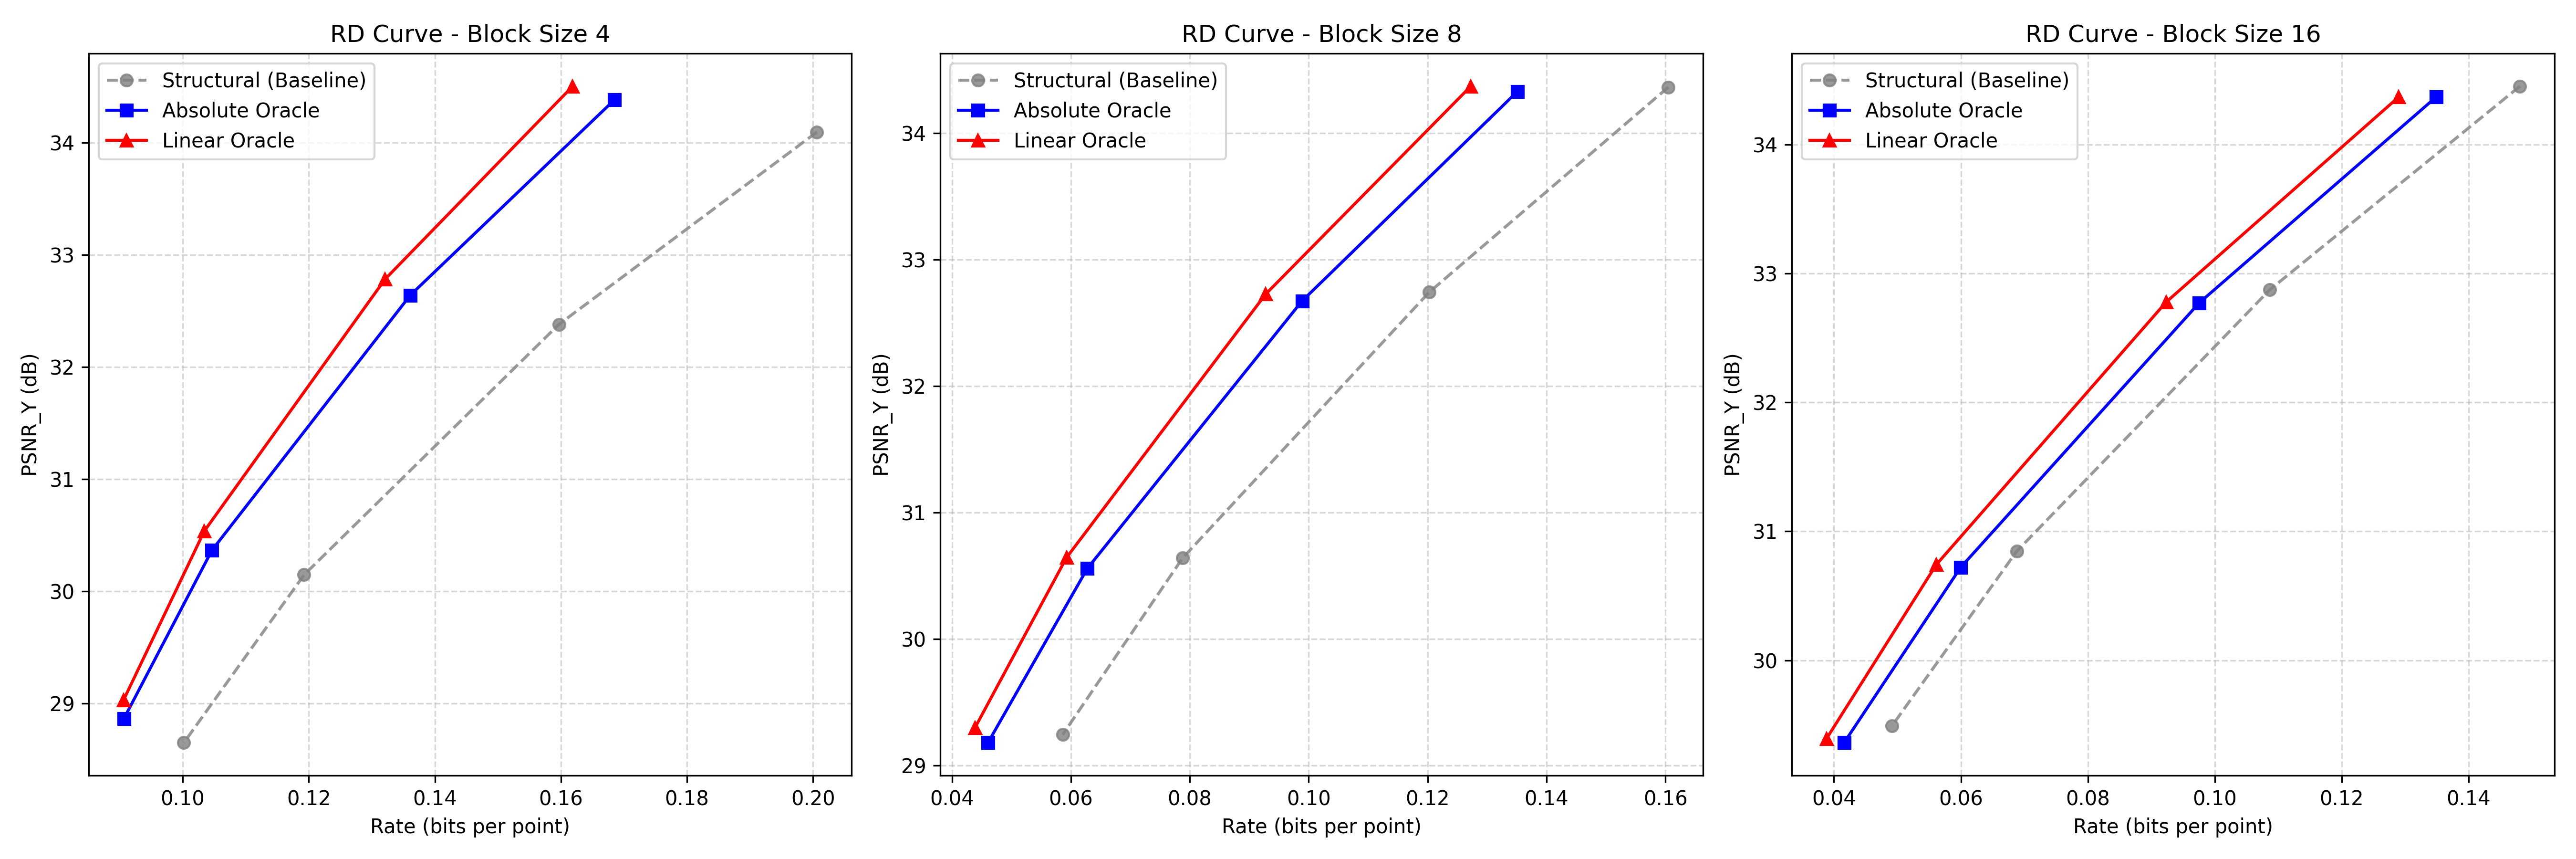
\includegraphics[width=1.0\linewidth]{img/resultados/rd_curves_comparison.png}
    \caption{Curvas Rate-Distortion para diferentes tamaños de bloque comparando la línea base con ambos oráculos.}
    \label{fig:rd_curves_oracle}
\end{figure}

\begin{figure}[ht]
    \centering
    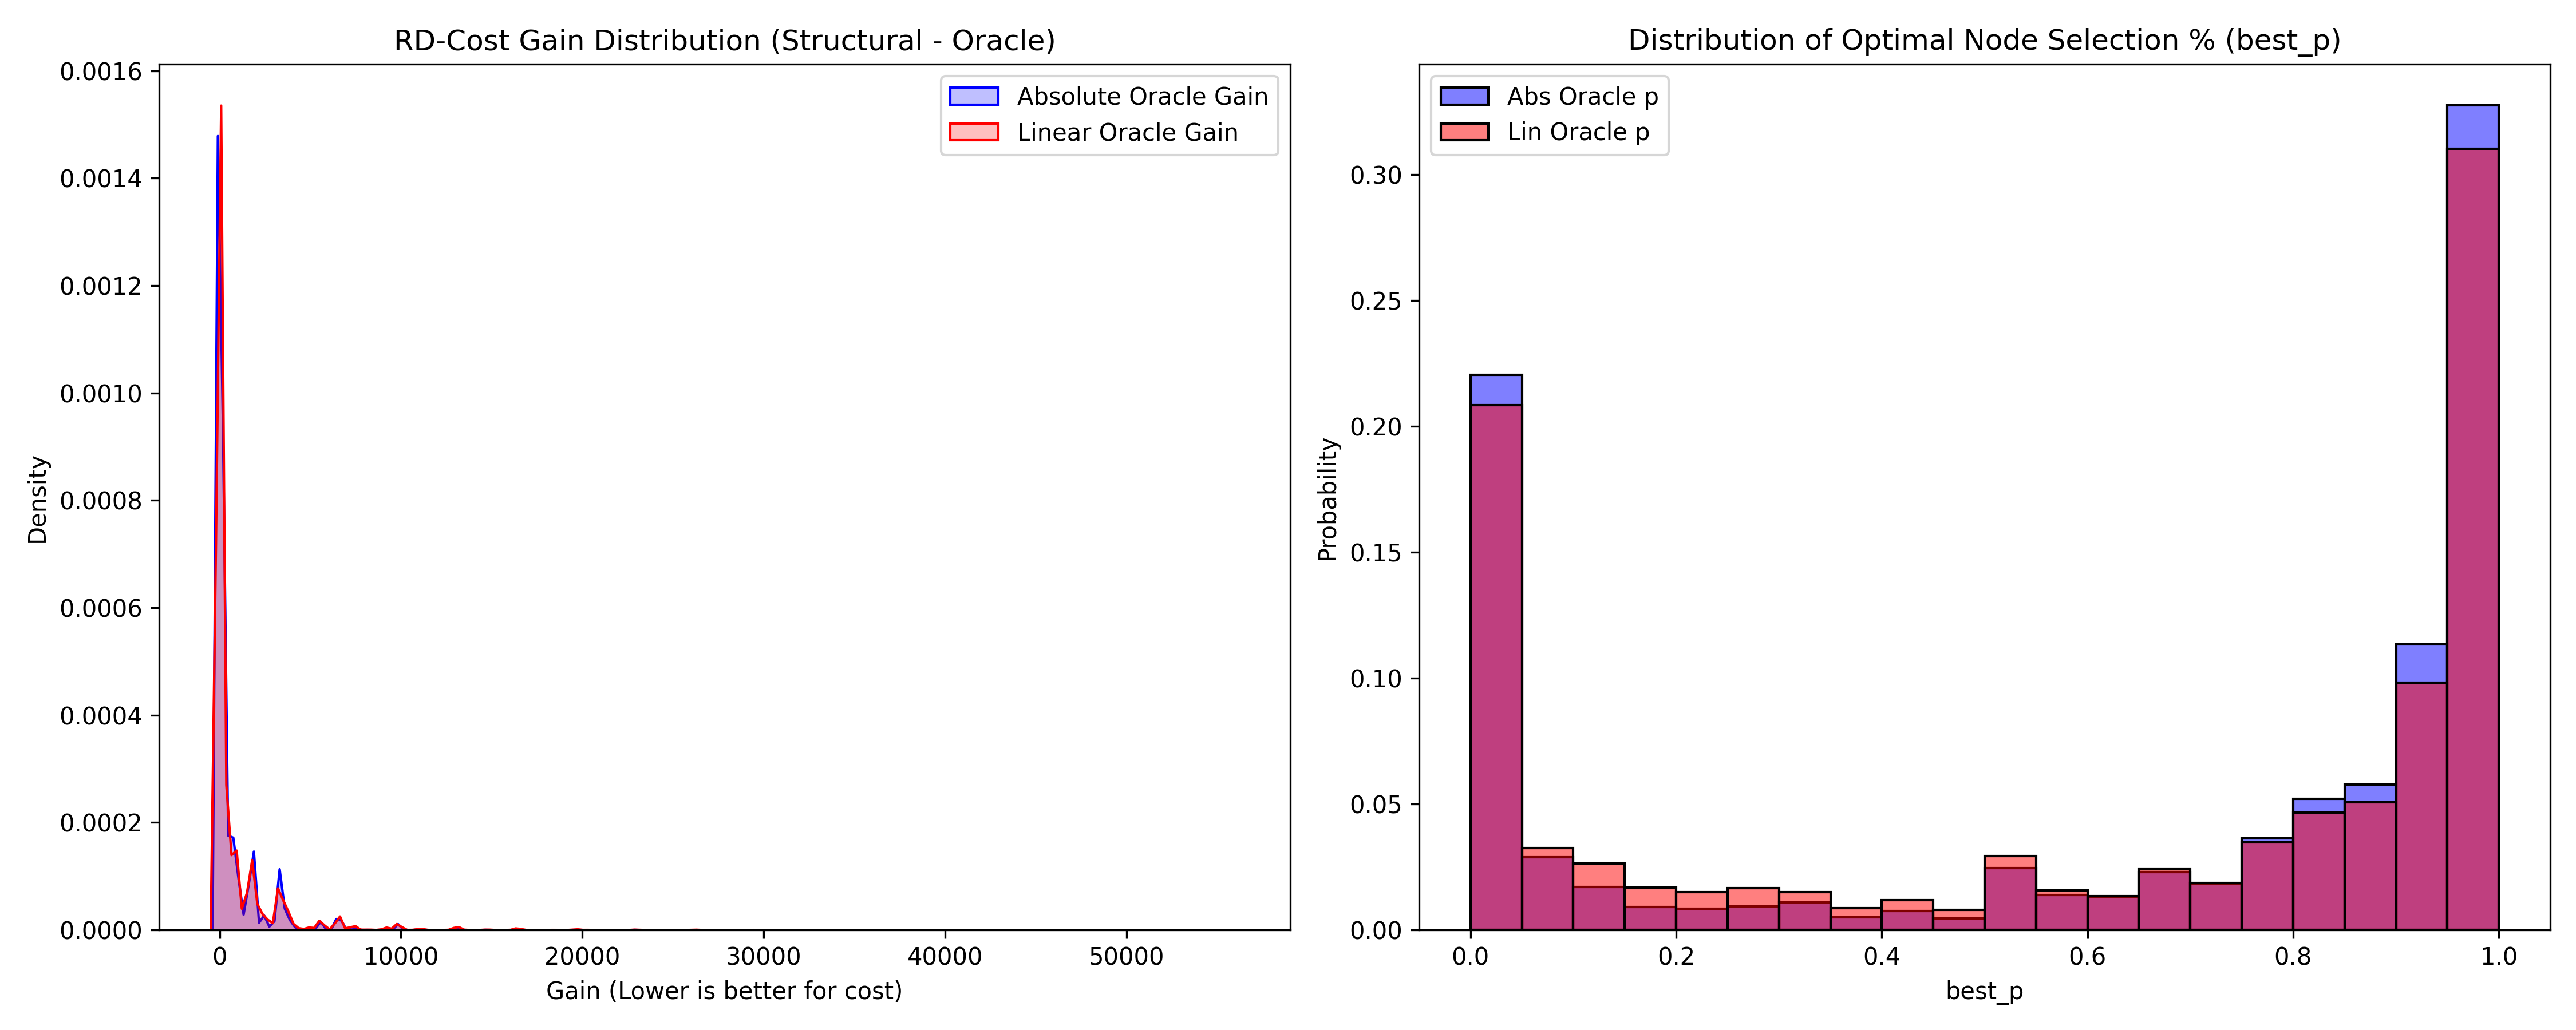
\includegraphics[width=0.8\linewidth]{img/resultados/gain_parameters_analysis.png}
    \caption{Análisis de distribución de ganancias y parámetros óptimos de selección de nodos ($p$).}
    \label{fig:gain_analysis}
\end{figure}

Como se observa en la Figura \ref{fig:gain_analysis}, la distribución de los parámetros óptimos se mantiene estable para ambas ejecuciones del oráculo. Esta consistencia es fundamental, ya que sugiere que el comportamiento del sistema no es errático ante diferentes aproximaciones de la señal. Por consiguiente, es viable realizar un paso posterior de agrupación (clustering) de estos parámetros, lo que permitiría una representación compacta de la configuración de adaptación con un overhead de señalización mínimo en el flujo de bits final.

\section{Análisis de Sensibilidad y Agrupamiento RD (RD-Clustering)}

En esta sección se presentan los resultados de la estrategia de agrupamiento conjunta de pendientes y parámetros de auto-lazo ($S_x, S_y, S_z, SLW, SLP$). El objetivo es evaluar la estabilidad del sistema, su capacidad de aprendizaje y los límites de saturación del libro de códigos.

\subsection{Saturación de Capacidad y Resolución Estructural}

Se evaluó el comportamiento del costo RD final en función del número de clusters ($C$) para diferentes tamaños de bloque.

\begin{figure}[ht]
    \centering
    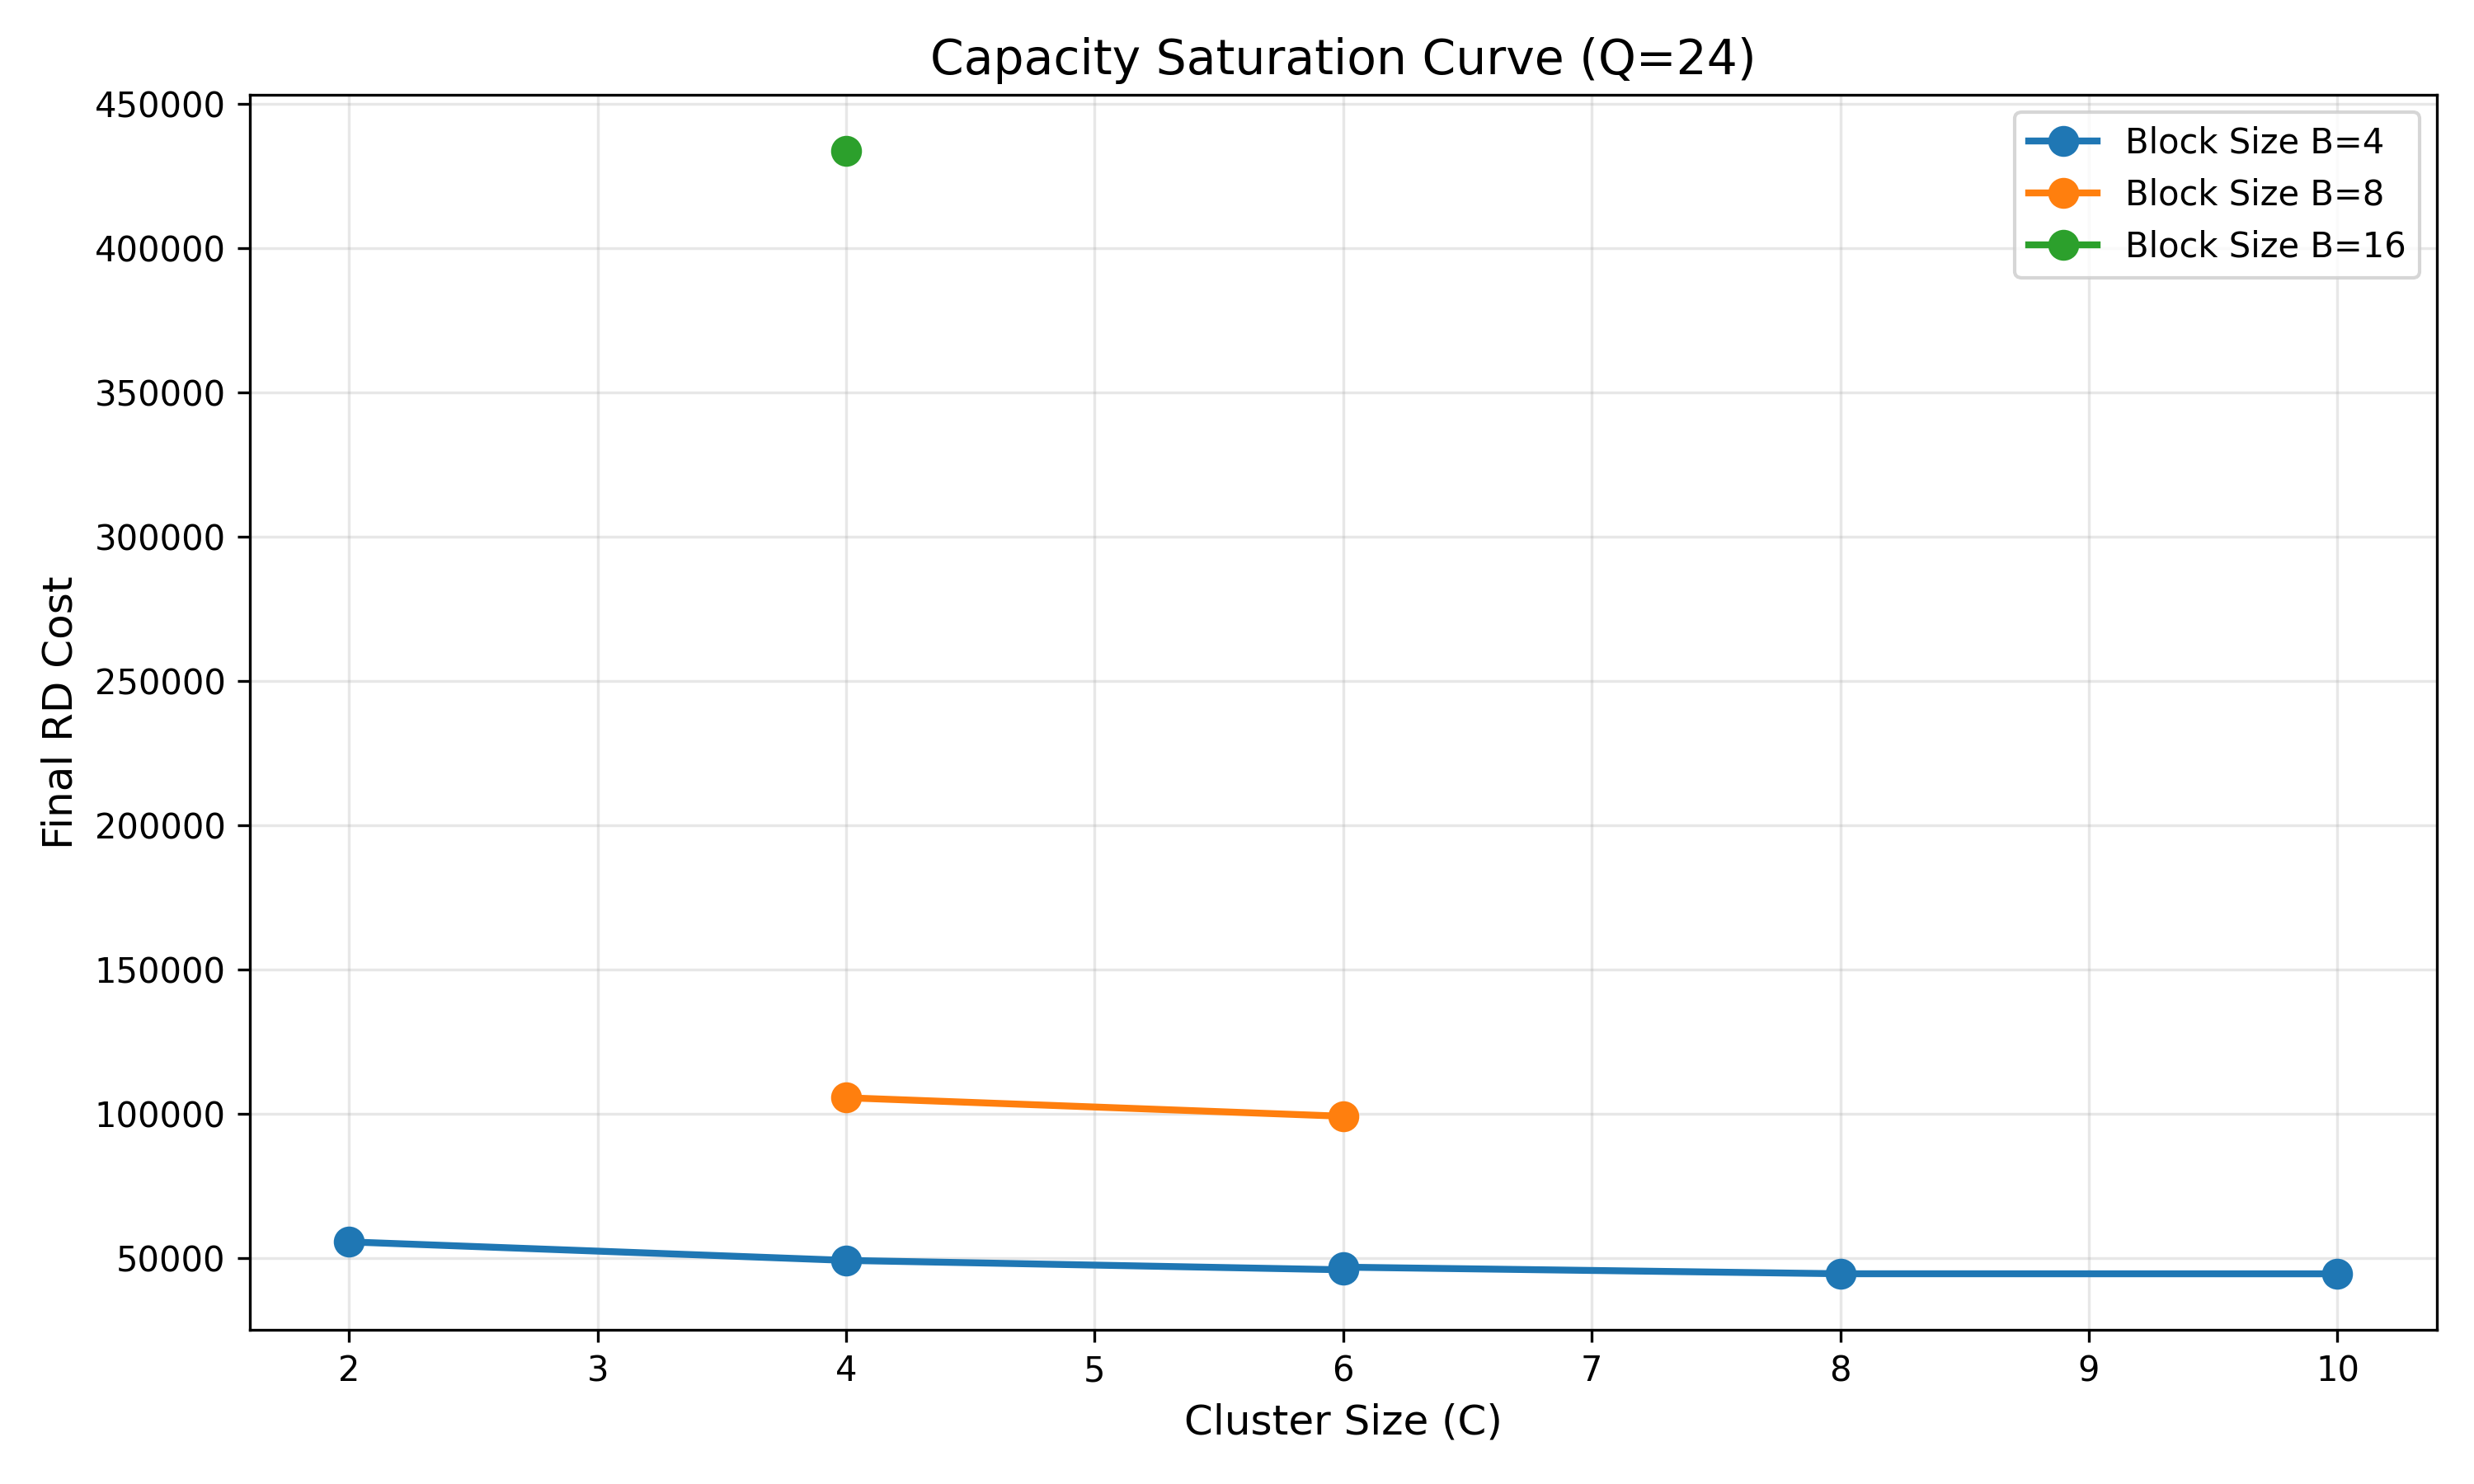
\includegraphics[width=0.8\linewidth]{img/resultados/capacity_saturation.png}
    \caption{Curva de saturación de capacidad para diferentes tamaños de bloque (Q=24).}
    \label{fig:capacity_saturation}
\end{figure}

% --- ESPACIO PARA ESCRITURA ---
% Sugerencia: Analizar cómo B=4 responde mejor al incremento de C y dónde se observa el plateau.


\subsection{Trayectoria de Aprendizaje y Sparsification del Grafo}

La evolución de los parámetros de auto-lazo durante el proceso iterativo revela la estrategia de optimización del sistema para reducir la tasa de bits.

\begin{figure}[ht]
    \centering
    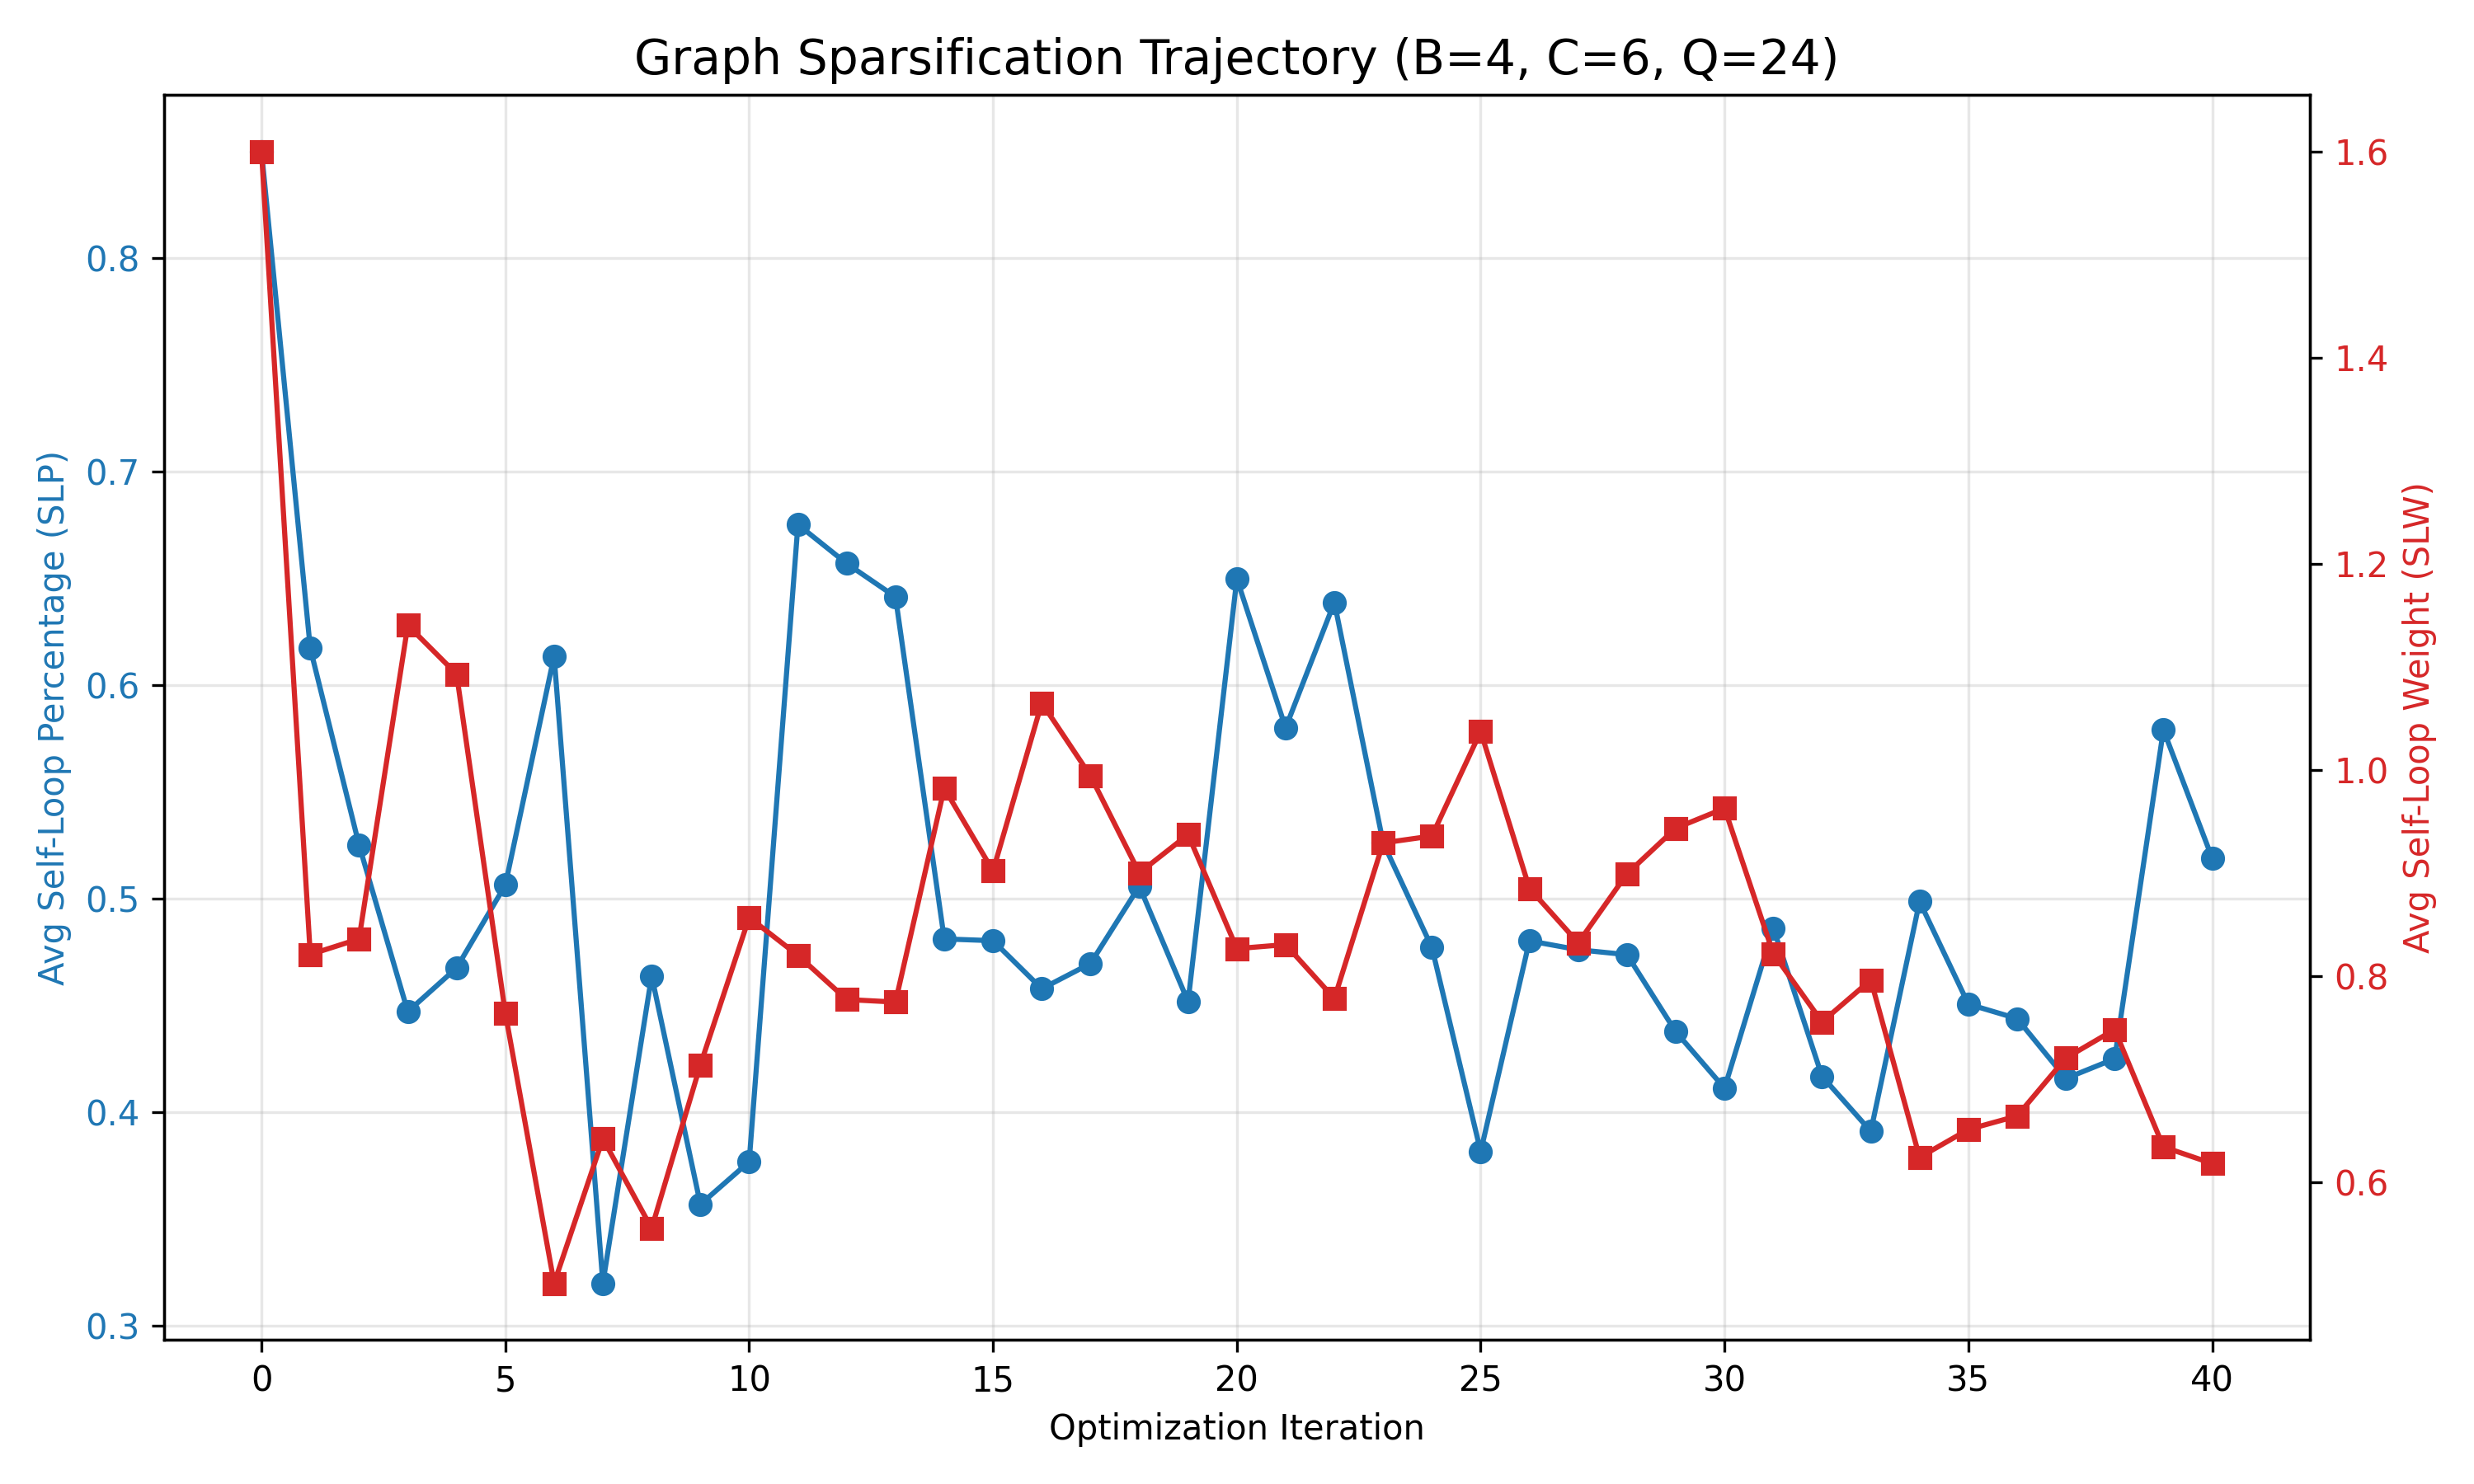
\includegraphics[width=0.8\linewidth]{img/resultados/parameter_drifts.png}
    \caption{Evolución temporal de los parámetros SLP y SLW (B=4, C=6, Q=24).}
    \label{fig:parameter_drifts}
\end{figure}

% --- ESPACIO PARA ESCRITURA ---
% Sugerencia: Comentar la caída drástica de SLP y qué significa para la conectividad del grafo.


\subsection{Velocidad de Convergencia e Impacto de la Inicialización}

Se analiza el esfuerzo de reasignación (distancia Hamming) y la velocidad con la que el sistema alcanza un estado estable.

\begin{figure}[ht]
    \centering
    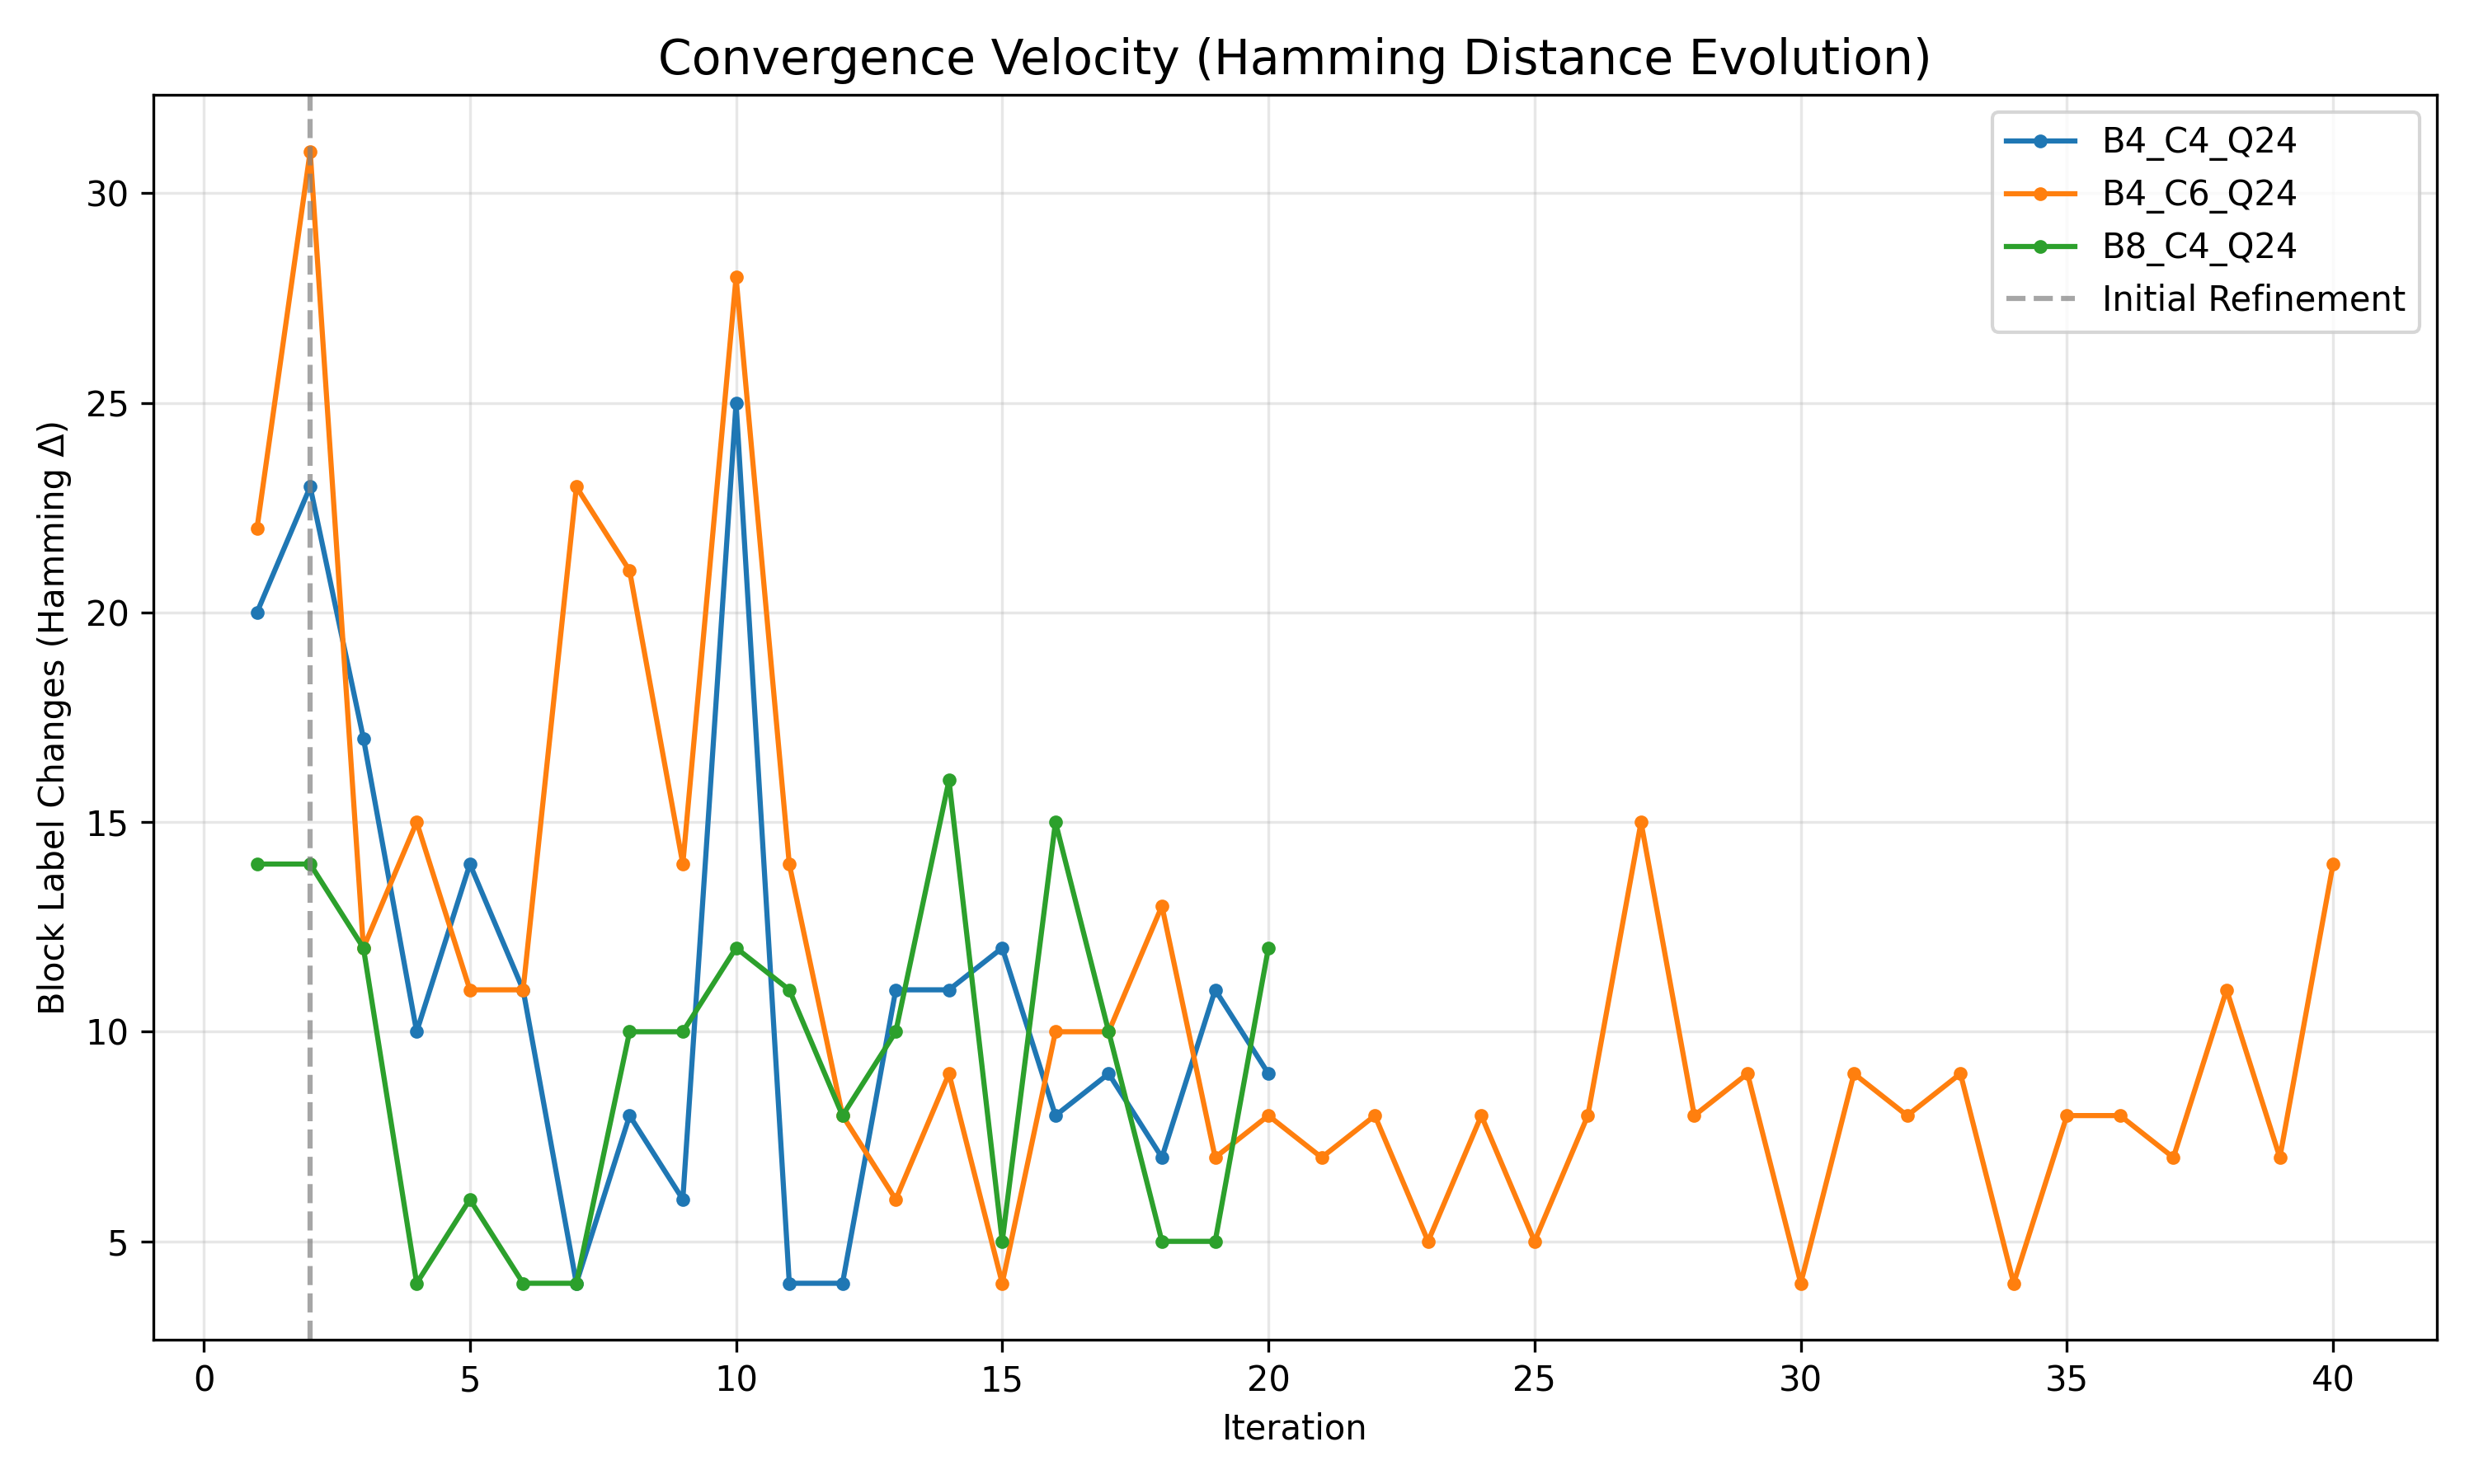
\includegraphics[width=0.8\linewidth]{img/resultados/convergence_velocity.png}
    \caption{Evolución de la distancia Hamming (reasignaciones de bloques) por iteración.}
    \label{fig:convergence_velocity}
\end{figure}

% --- ESPACIO PARA ESCRITURA ---
% Sugerencia: Describir el "Iter 2 Breakthrough" y la persistencia de cambios en configuraciones complejas.


\subsection{Frontera de Eficiencia Informacional}

Finalmente, se mapea la relación entre la ganancia obtenida y el costo de señalización (entropía) requerido para transmitir los índices de los clusters.

\begin{figure}[ht]
    \centering
    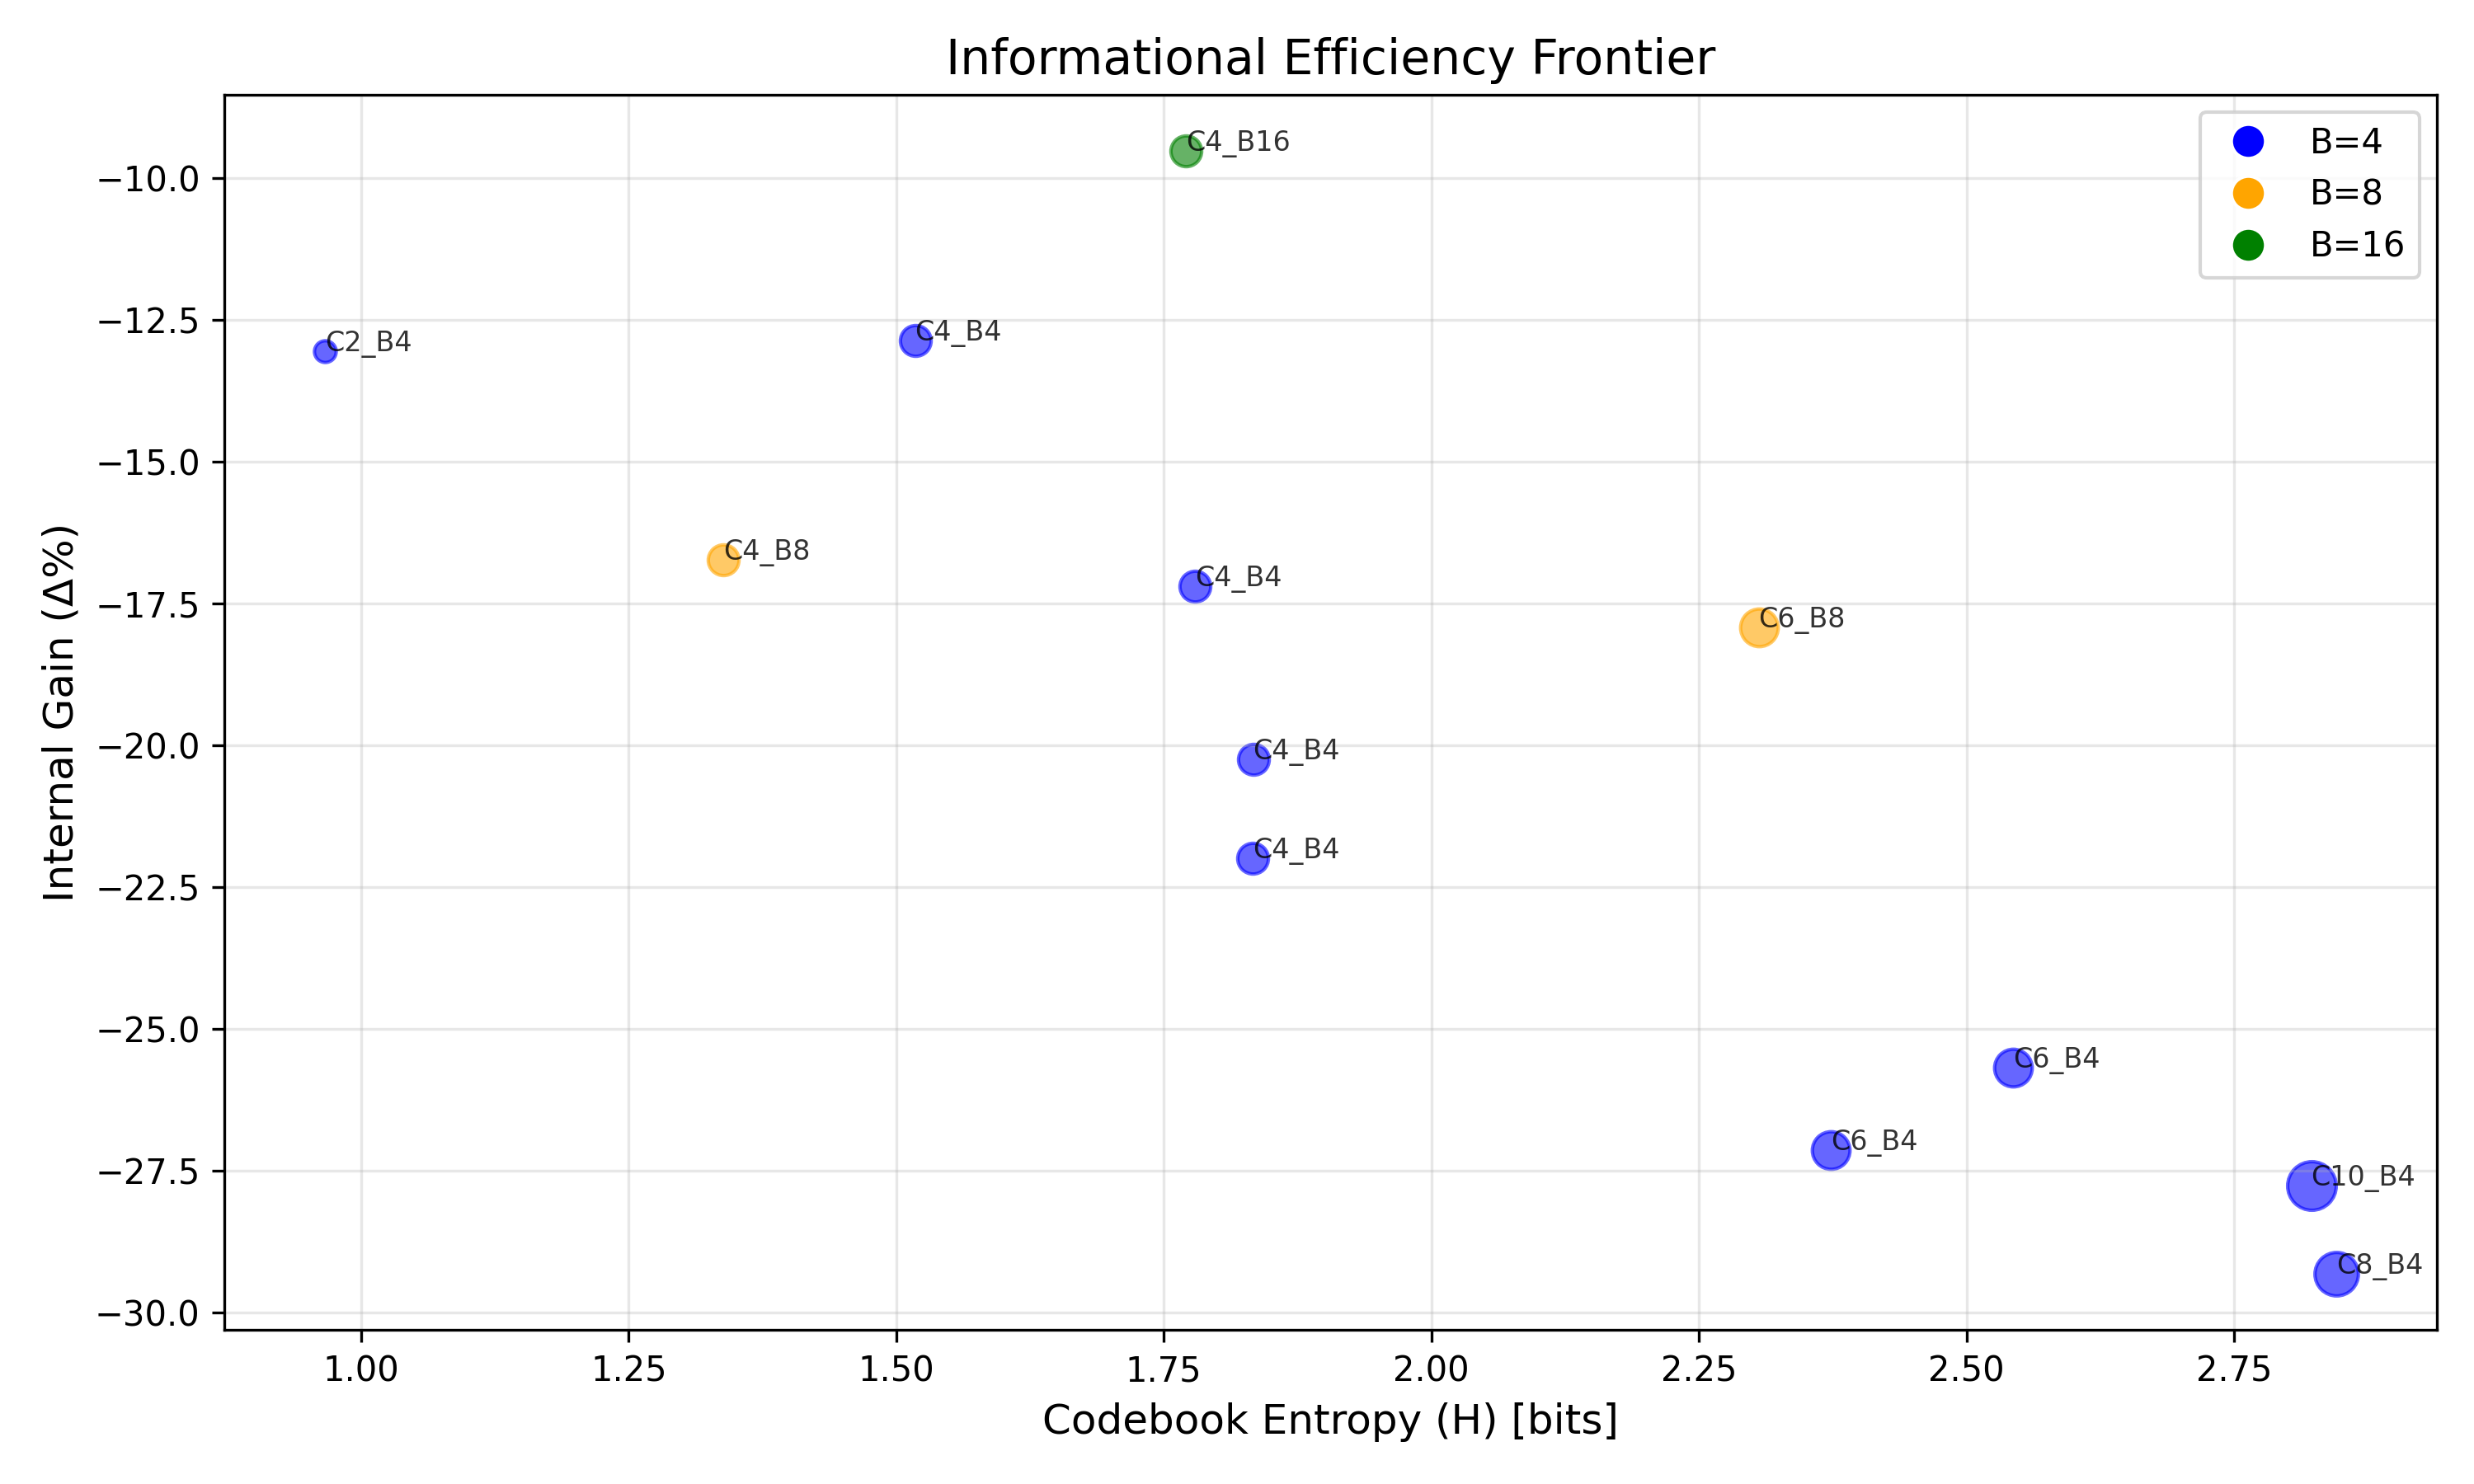
\includegraphics[width=0.8\linewidth]{img/resultados/efficiency_frontier.png}
    \caption{Frontera de Pareto: Entropía del libro de códigos vs. Ganancia Interna.}
    \label{fig:efficiency_frontier}
\end{figure}

% --- ESPACIO PARA ESCRITURA ---
% Sugerencia: Discutir qué configuraciones (C, B) ofrecen la mejor relación ganancia/overhead.


%
\bibliography{library}
% FIN DEL DOCUMENTO
\end{document}